\newpage % Rozdziały zaczynamy od nowej strony.
\section{Rozwiązanie}

W tym rozdziale przedstawione zostaną wybrane metody, które zostały sprawdzone w ramach analizy problemu. Rozważania zostaną przedstawione w ścisłym związku z pytaniami badawczymi przedstawionymi w celu pracy, a więc:

\begin{itemize}
    \item Jak można zaprojektować model oparty na głębokim uczeniu do wspólnej segmentacji semantycznej i klasyfikacji scen w środowiskach wewnętrznych?
    \item Czy przestrzeń reprezentacji po wytrenowaniu na zadaniu segmentacji semantycznej może być użyta do zadania klasyfikacji sceny?
    \item Jak dobrze proponowany model radzi sobie na dużym zbiorze danych scen wewnętrznych i jak wypada w porównaniu z aktualnymi metodami segmentacji semantycznej i klasyfikacji scen osobno?
    \item Jak proponowany model może być wykorzystany do poprawy wydajności w robotyce mobilnej?
\end{itemize}
Opis rozwiązań problemu zostanie poprzedzony przeglądem rozwiązań. Analiza dotychczasowego stanu wiedzy pozwoli lepiej ukierunkować badania. Intuicja oraz wskazówki zdobyte podczas przeglądu zostaną uwzględnione w doborze metod i eksperymentów.

\subsection{Przegląd rozwiązań}
Przegląd literatury jest kluczowym aspektem każdej pracy naukowej. W tym podrozdziale zostaną przedstawione wyłącznie rozwiązania obejmujące łączną segmentację semantyczną oraz klasyfikację sceny. Szczególny nacisk położony zostanie na architektury głębokich, wielozadaniowych sieci neuronowych. Niestety przyjęte założenia w pracy nie zostały opisane przez nikogo wcześniej, zgodnie z najlepszą wiedzą autora. Niektóre prace naukowe przedstawiają ten sam problem, to jest klasyfikacji i segmentacji łącznie, ale obejmują go w innej domenie danych. Z drugiej strony artykuły obejmujące środowiska wnętrz są dobrze zdefiniowane, jednak często w swoich rozwiązaniach autorzy korzystają z obrazu głębi, który nie zawiera się w zakresie badań tej pracy. Nie mniej wszystkie poniższe artykuły stanowią cenne źródło informacji oraz wskazówek.

\vspace{0.5cm}

Pierwszym z prezentowanych artykułów jest ,,Describing the Scene as a Whole: Joint Object Detection, Scene Classification and Semantic Segmentation'' autorstwa Yao J. et al. (2012)\cite{yao2012describing}. Prezentuje on algorytm, który ówcześnie wyznaczył najlepsze podejście (ang. state-of-the-art (SOTA)). Rozwiązanie opiera się na warunkowych polach losowych, które ówcześnie były szeroko stosowane. Mimo że nie jest to rozwiązanie oparte o głębokie sieci neuronowe, to autorzy wskazują tutaj ważne zagadnienia. Po pierwsze udowadniają, że połączenie segmentacji i klasyfikacji okazało się owocne nie tylko pod względem jakości, ale również wydajności w kontekście czasowym. W swojej pracy wykorzystują podejście równolegle zgodne z rysunkiem \ref{fig:scene-as-a-whole}. Podsumowując, ,,Describing the Scene as a Whole: Joint Object Detection, Scene Classification and Semantic Segmentation'' nie jest propozycją architektury głębokiej sieci. Wskazuje on na problemy z łączeniem zadań szeregowo, jednocześnie udowadniając, że taka praktyka był ówcześnie stosowana, więc nie można uznawać stosowania połączenia szeregowego jako niedopuszczalnego. Poza tym autorzy doceniają wspólne realizowanie zadań, oceniając je jako bardziej efektywne czasowo i obliczeniowo.

\begin{figure}[ht!]
    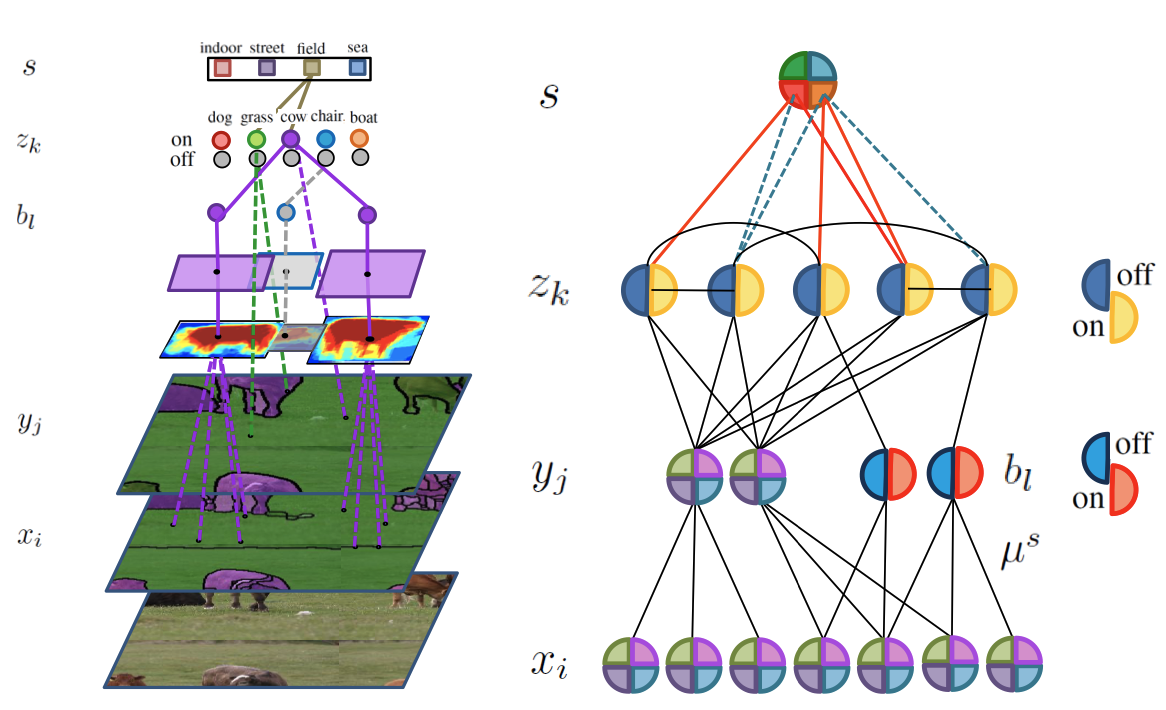
\includegraphics[width=\textwidth]{img/joint-segmentation-and-classification.png}
    \caption{Describing the Scene as a Whole: Joint Object Detection, Scene Classification and Semantic Segmentation (2012) \cite{yao2012describing}.}
    \label{fig:scene-as-a-whole}
\end{figure}
\vspace{0.5cm}
Artykuł ,,Let there be Color!: Joint End-to-end Learning of Global and Local Image Priors for Automatic Image Colorization with Simultaneous Classification'' (2016) \cite{iizuka2016let} przedstawia rozwiązanie problemu jednoczesnego klasyfikowania sceny oraz kolorowania zdjęć. Do realizacji zadania kolorowania potrzebna jest semantyczna maska. Wynika z tego, że kolorowanie jest rozszerzeniem segmentacji semantycznej. Rozumiejąc towarzyszące analogie, można przejść do analizy rozwiązania. Przedstawiona architektura (rys.\ref{fig:parrarel-arch}) jest przykładem sieci wielozadaniowej, używającej miękkiego dzielenia parametrów, ale tylko i wyłącznie w obrębie pierwszej części sieci. Szczególnie ciekawa jest konkatenacja cech wysokiego poziomu (Global Features Network) z cechami średniopoziomowymi (Mid-Level Features Network), która ma miejsce w warstwie fuzji (Fusion layer). Iizuka et al. formułują wniosek oznajmiający o kluczowym znaczeniu tej warstwy w kontekście całego zadania. Wiedza o scenie zdjęcia może dostarczyć informacji wpływających na decyzję, czy na obrazie znajduje się niebo, czy trawa. Rozważając sceny wnętrz, oczywiste jest, że nie będzie tam takich grup semantycznych, jednak bezpośrednia informacji o miejscu sceny, np. łazienka, może pomóc w ustaleniu etykiet segmentacji. Podsumowując, cechy nauczone na zadaniach klasyfikacji i segmentacji, mogą wzajemnie pozytywnie na siebie wpływać, realizując pozytywny transfer.
\begin{figure}[ht!]
    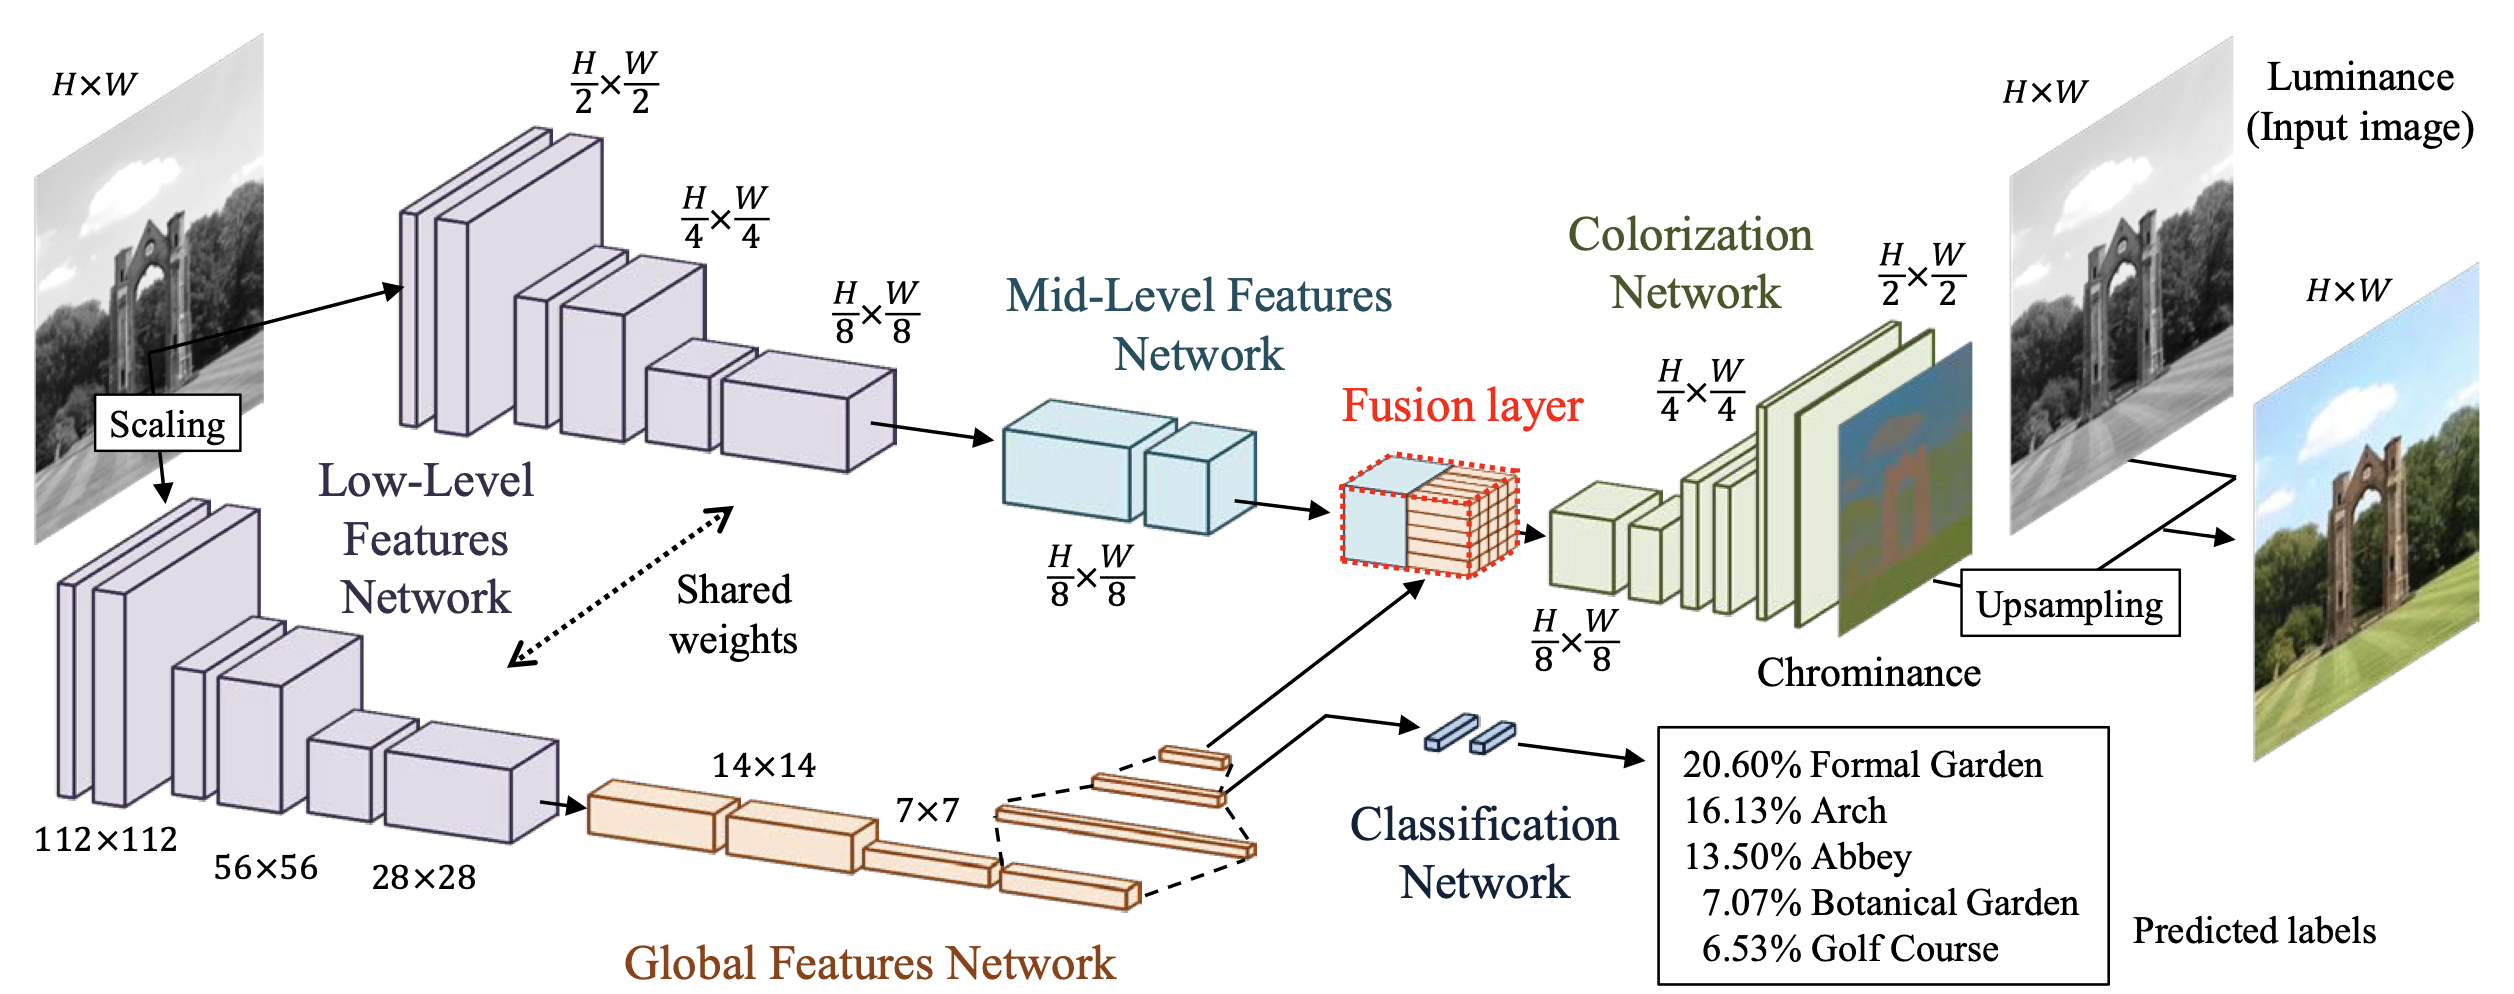
\includegraphics[width=\textwidth]{global-local-features.png}
    \caption{Let there be Color!: Joint End-to-end Learning of Global and Local Image Priors for Automatic Image Colorization with Simultaneous Classification 2016 \cite{iizuka2016let}.}
    \label{fig:parrarel-arch}
\end{figure}


\vspace{0.5cm}
Zastosowanie łącznej segmentacji oraz klasyfikacji tym razem w domenie obrazowania medycznego przedstawia ,,Y-Net: Joint Segmentation and Classification for Diagnosis of Breast Biopsy Images'' (2018) \cite{mehta2018net}. Zadania te są realizowane przez twarde dzielenie parametrów w kontekście uczenia wielozadaniowego (rys. \ref{fig:y-net}). Architektura jest prostym rozszerzeniem klasycznego U-Netu. Autorzy wskazują, że taki zabieg powoduje dużą modularność, ponieważ do dowolnego modelu segmentacji można podłączyć sieć klasyfikacyjną. Przeprowadzone eksperymenty dla segmentacji udowodniły, że dokładność pozostała na tym samym poziomie. W przypadku klasyfikacji wyniki były wyższe niż dotychczasowe SOTA na tym zbiorze. Jako funkcję straty autorzy użyli sumy entropii skrośnej każdego z zadań. Podsumowując, zadanie segmentacji osiągnęło ten sam wysoki wynik co SOTA, a zadanie klasyfikacji ustanowiło nowe SOTA na tym zbiorze, ucząc się znacznie mniej parametrów.


\begin{figure}[ht!]
    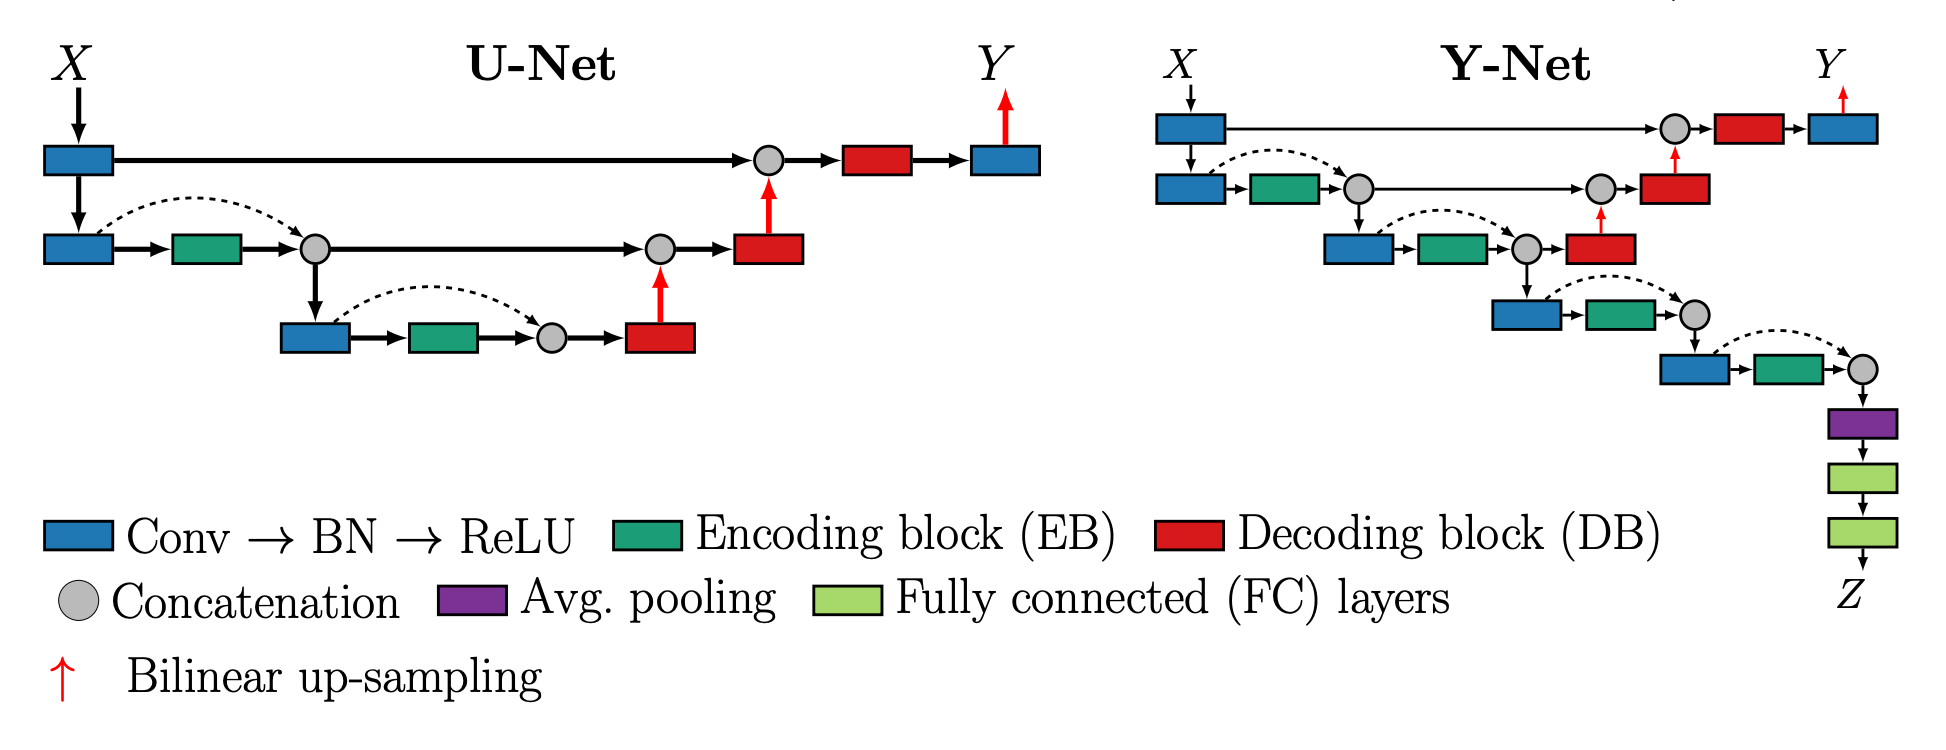
\includegraphics[width=\textwidth]{y-net-new.png}
    \caption{Y-Net: Joint Segmentation and Classification for Diagnosis of Breast Biopsy Images 2018 \cite{mehta2018net}.}
    \label{fig:y-net}
\end{figure}

\vspace{0.5cm}

Najbliższym artykułem tej pracy inżynierskiej jest ,,Efficient Multi-Task RGB-D Scene Analysis for Indoor Environments'' (2022) \cite{9892852}, który został opublikowany w czasie tworzenia tej pracy. Przedstawia on jedną głęboką sieć neuronową rozwiązującą następujące zadania: segmentacja semantyczna oraz segmentacja instancji (łącznie ang. pantopic segmentation), estymacja orientacji instancji oraz klasyfikacja sceny. Rozważaną przez autorów domeną są podobnie jak w przypadku tej pracy sceny wnętrz. Znaczną różnica poza dodatkowymi zadaniami jest użycie przez Seichter et al. informacji o głębi. Zgodnie z wnioskami z niniejszego artykułu przetwarzanie łączne obrazów RGB i głębi jest kluczowe z punktu widzenia jakości predykcji, więc nie można bezpośrednio porównać go z niniejszą pracą. Autorzy wykonali wiele eksperymentów, badając różne metodologie. Architektura jest przedstawiona na rysunku \ref{fig:emsanet}. Autorzy zdecydowali się na twarde dzielenie parametrów, argumentując całkowitą niezależnością w przypadku chęci wyłączenia jednego zadań z wnioskowania. Pierwszym krokiem, który wykonali, było ustalenie punktu odniesienia poprzez trenowanie osobno każdego z zadań. Trening każdej sieci z osobna był rozważany pod względem wielu backbone'ów ze zróżnicowaniem na uczenie wyłącznie obrazu głębi, obrazu RGB lub RGB-D. Z reguły w przypadku segmentacji oraz klasyfikacji większy backbone wpływał na polepszenie wyników. Trenując zadania łącznie, zdecydowano się na ważoną sumę entropii skrośnej dla zadania segmentacji i klasyfikacji w proporcjach odpowiednio 3:1. Przyjęty krok uczenia, będąc sprawdzonym przez przeszukiwanie liniowe (ang. grid search), jest wyjątkowo duży, bo wynosi 0.02. Autorzy zastosowali zaawansowane techniki dostosowywania kroku uczenia w trakcie treningu poprzez użycie planisty polityki jednego cyklu (ang. one cycle policy scheduler). Jako optymalizator użyto SGD z momentem oraz drobną regularyzacją. Podsumowując, zgodnie z prezentowanymi wynikami na wspólnej segmentacji oraz klasyfikacji autorom nie udało się polepszyć działania modelu na segmentacji semantycznej. Z powodzeniem jednak wzrosła dokładność klasyfikacji na zbiorze NYUv2.

\begin{figure}[ht!]
    \centering
    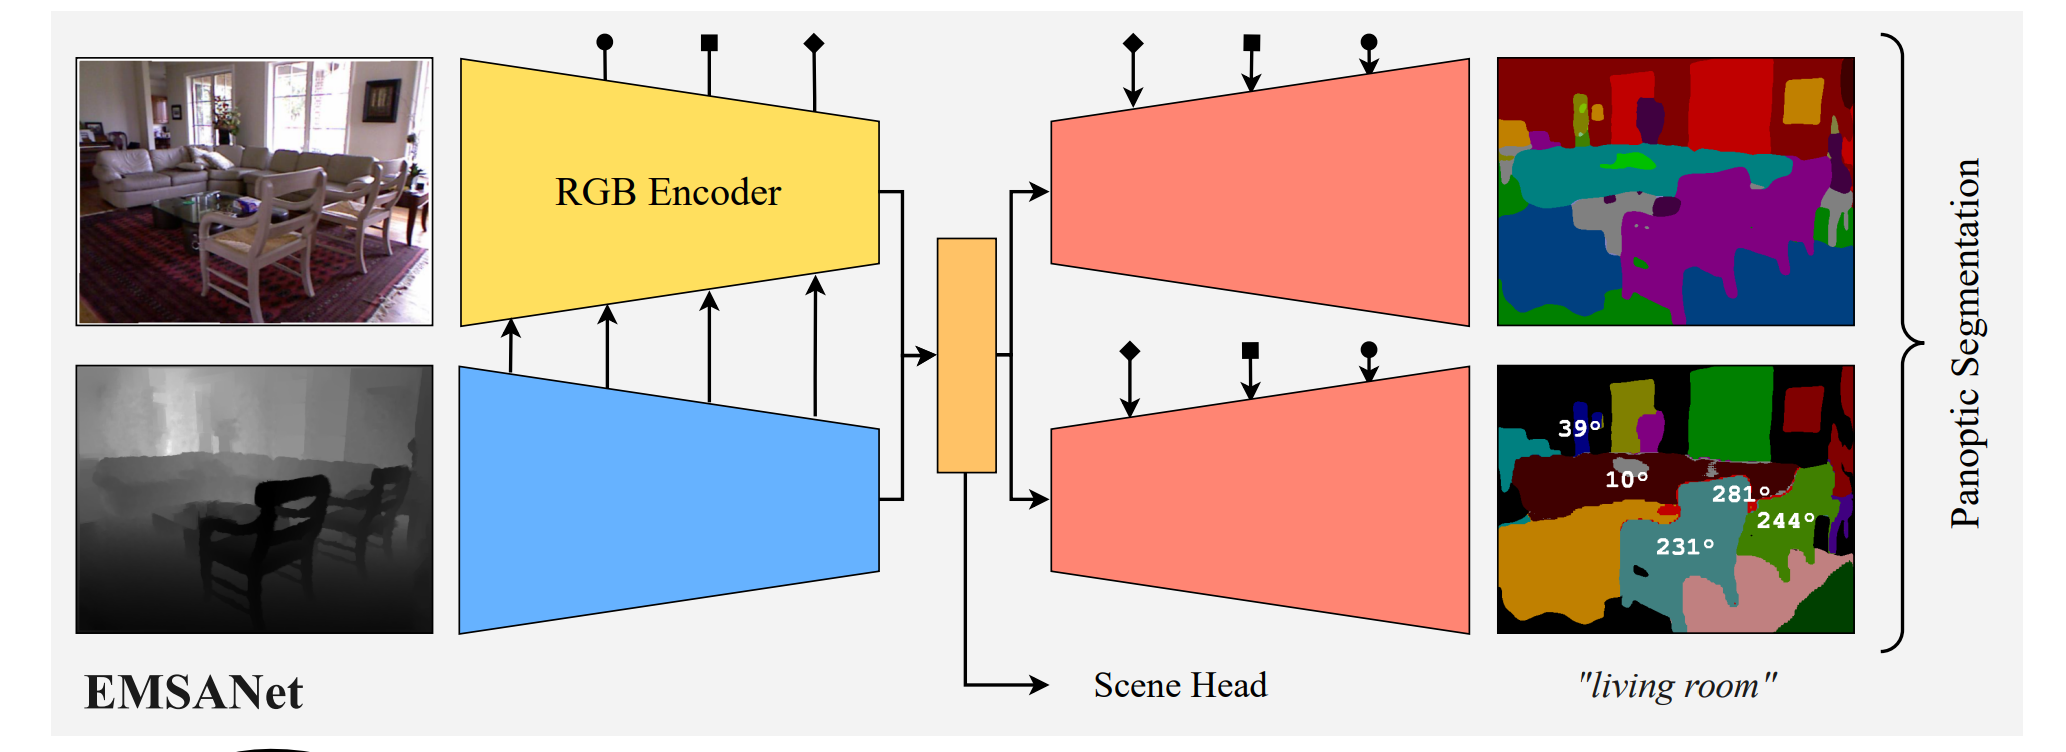
\includegraphics[width=\textwidth]{emsanet.png}
    \caption{Efficient Multi-Task RGB-D Scene Analysis for Indoor Environments \cite{9892852}}
    \label{fig:emsanet}
\end{figure}


\subsubsection{DeepLabV3}
Literatura uważa go za model lepszy od sieci U-Net czy FCN. Model DeepLabV3 nie korzysta z połączeń pomijających. Informacje o kontekście w wielu skalach uzyskuje przez moduł Spatial Pyramid Pooling (SPP). Wykorzystuje on bloki Atrous Spatial Pyramid Pooling (ASPP) oraz klasyczny pooling. Bloki ASPP składają się ze splotu, normalizacji pakietowej oraz funkcji aktywacji ReLU. Sploty przyjmują różną postać. Pierwszy blok to splot o jądrze 1x1. Następne bloki korzystają z rozszerzonego splotu o dylatacji oraz wypełnieniu (padding) równemu współczynnikowi rozszerzenia (dilatation rate). Dla kolejnych 3 bloków wynosi on 12, 24, 36. Ostatni blok SPP to zwykły pooling. Bloki składające się na moduł SPP są następnie dodawane wzdłużnie i poddawane splotowi. Następnie egzekwuje się splot o wyjściowej liczbie kanałów równej ilości klas. Końcowy etap obejmuje upsampling do pożądanego wymiaru.
\begin{figure}[ht!]
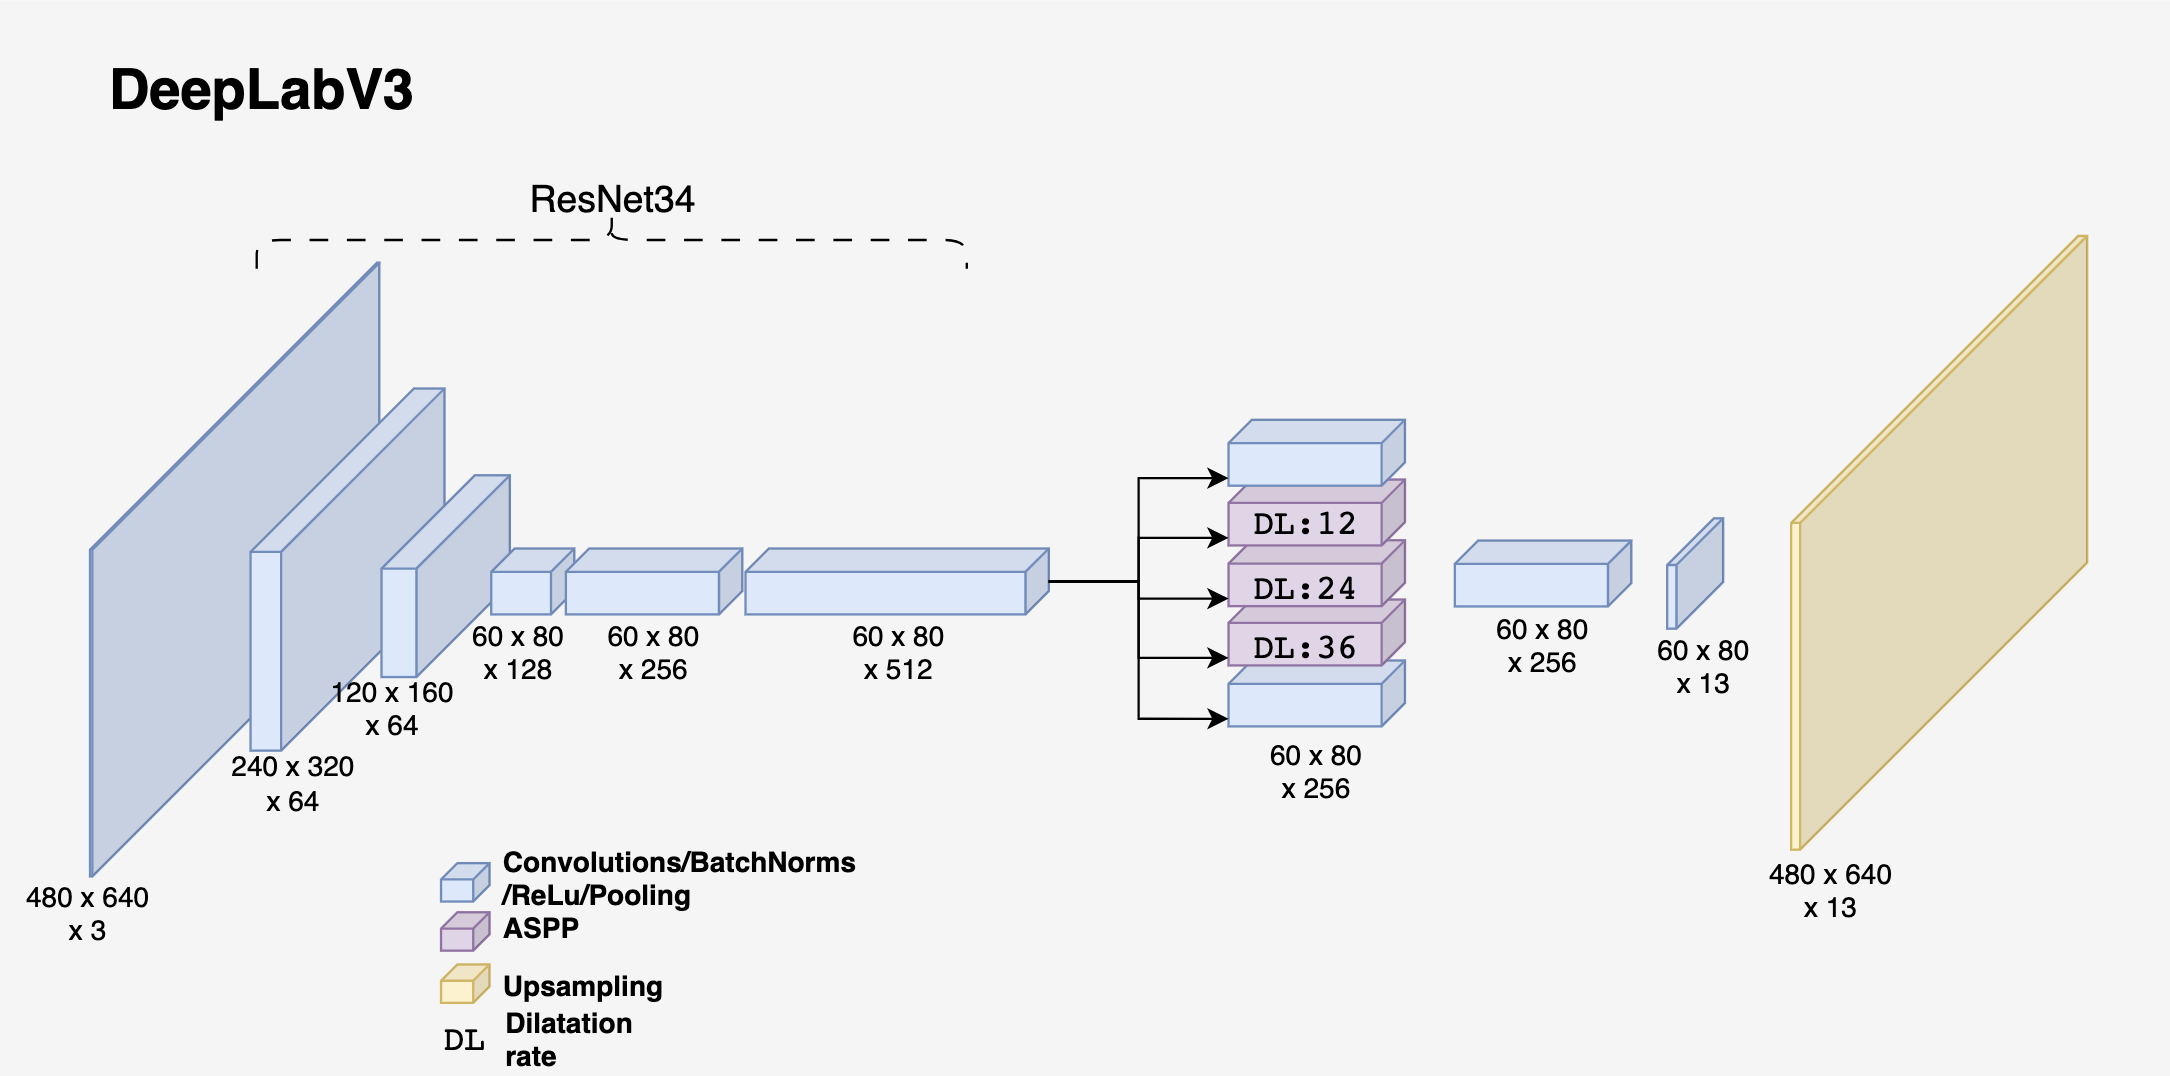
\includegraphics[width=\textwidth]{deeplabv3-new.png}
\caption{Klasyczna architektura DeepLabV3 z backbonem ResNet34.}
\label{fig:deeplabv3}
\end{figure}
\subsection{Rozwiązanie problemu}
W tym podrozdziale zostaną przedstawione eksperymenty, które wykonano w celu zbadania uczenia wielozadaniowego segmentacji semantycznej oraz klasyfikacji sceny w domenie pomieszczeń. Pierwszym etapem, jakiego dokonano, było wyznaczenie punktu odniesienia. Z punktu widzenia pracy najłatwiej byłoby znaleźć gotowe wyniki segmentacji oraz klasyfikacji sceny na wybranym zbiorze danych. Niestety żadne z przytaczanych rozwiązań nie odpowiada w pełni zakresowi pracy. Postanowiono stworzyć taki punkt odniesienia samemu przez analogiczne trenowanie sieci segmentacyjnej oraz klasyfikacyjnej osobno.

Mając taką wiedzę, eksperymentowano dalej z różnymi architekturami uczenia wielozadaniowego. Wybrano uczenie łączne o twardym dzieleniu parametrów. Podejście to ma wiele zalet. \cite{mehta2018net} podkreśla łatwość i wszechstronność implementacji. Wystarczy dołączyć do modelu część klasyfikacyjną. Co więcej, wszyscy autorzy (\cite{mehta2018net}, \cite{9892852}) chwalą znacznie mniejszą ilość parametrów sieci, co bezpośrednio wpływa na czas treningu oraz wnioskowania. Architektura sieci przedstawia rys. \ref{fig:multitask}. Jest to DeepLabv3 rozszerzony za enkoderem o sieć klasyfikacyjną podobnie jak w artykule \cite{mehta2018net}, gdzie rozszerzono sieć U-Net.

\begin{figure}[ht!]
\centering
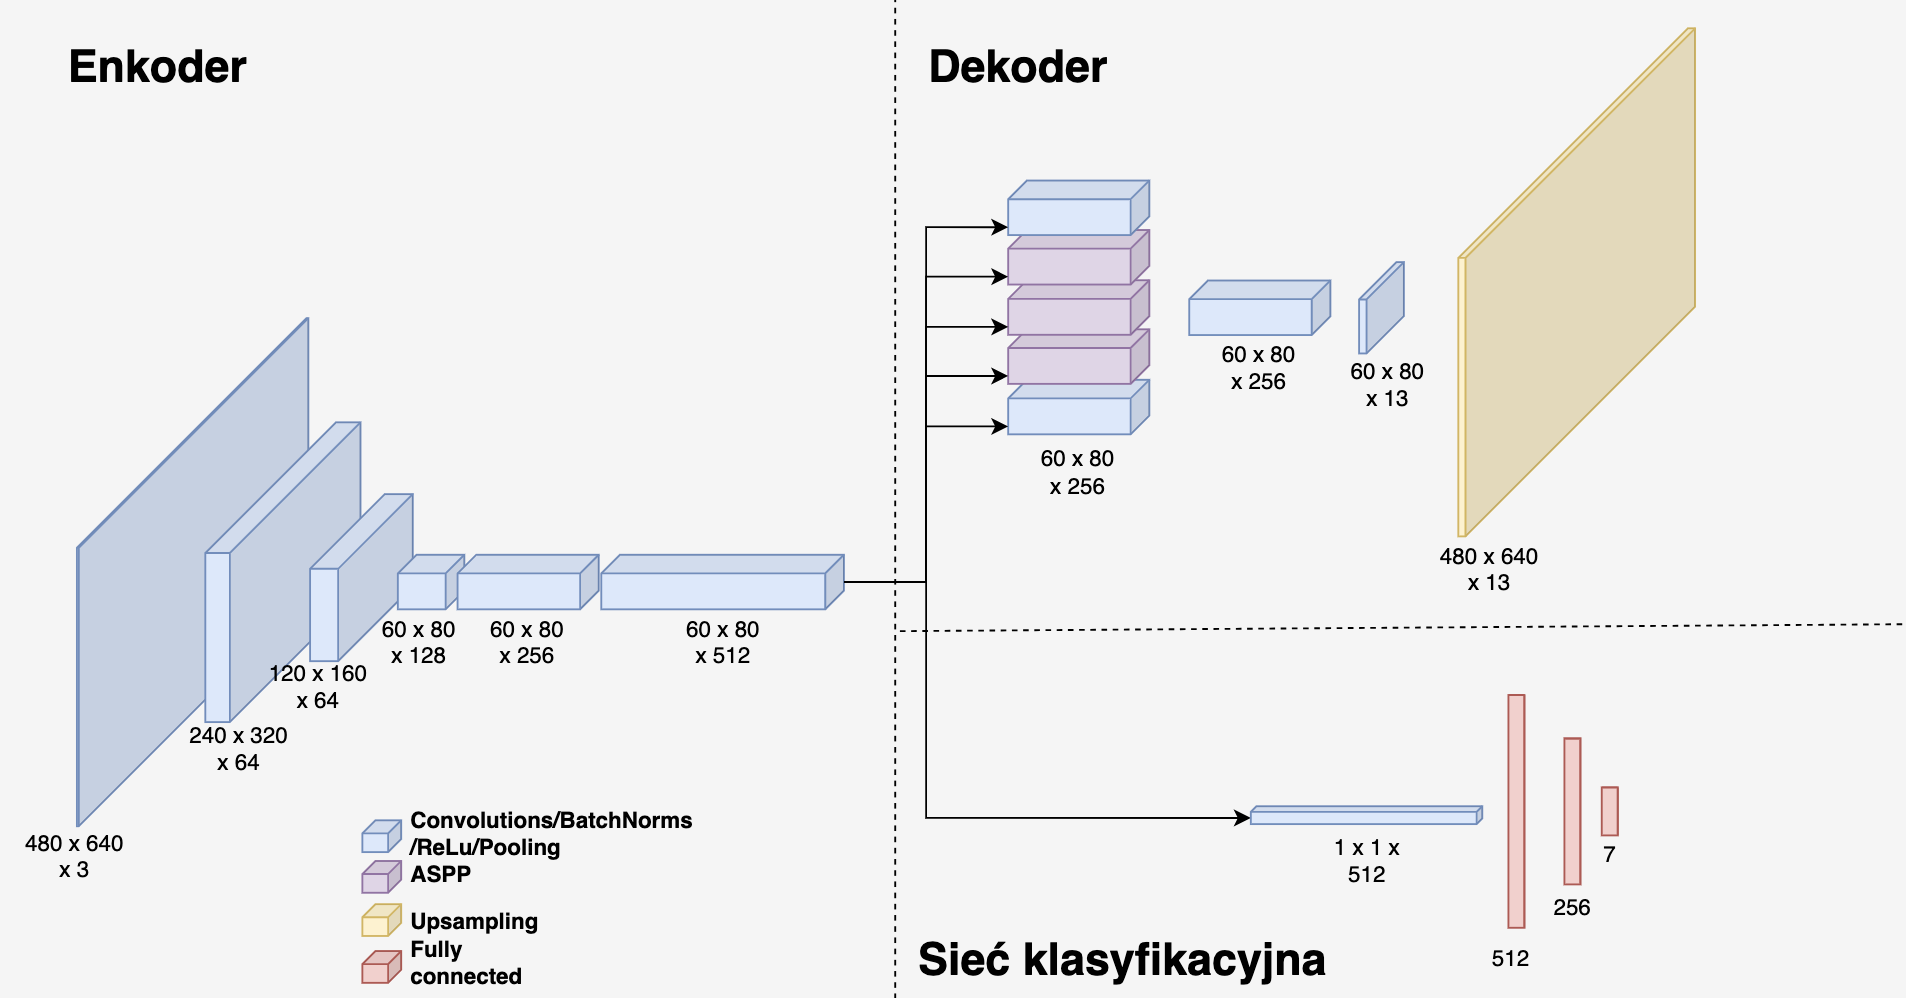
\includegraphics[width=\textwidth]{multitask-arch-new.png}
\caption{Architektura wielozadaniowej sieci.}
\label{fig:multitask}
\end{figure}

Normalizacja jest ważnym krokiem przetwarzania wstępnego w problemach widzenia komputerowego. W pracy ,,Normalization Techniques in Training DNNs: Methodology, Analysis and Application'' Lei et. al. \cite{huang2020normalization}, autorzy udowadniają, że normalizacja stabilizuje i przyśpiesza trening oraz prawdopodobnie prowadzi do poprawy generalizacji. Jako przetwarzanie wstępne obrazu zastosowano normalizację gaussowską. Obrazy RGB zostały poddane normalizacji ze średnią (0.485, 0.456, 0.406) oraz odchyleniem standardowym (0.229, 0.224, 0.225), które odpowiadają parametrom rozkładu normalnego na zbiorze ImageNet. Gotowe wagi uzyskane poprzez uczenie na bazie ImageNet służyły jako wagi początkowe enkodera.

Znalezienie optymalnego zestawu hiperparametrów nie jest proste. Niewłaściwy dobór grozi brakiem osiągnięcia pożądanych rezultatów. W celu pozyskania optymalnego zestawu skorzystano z narzędzia Optuna \cite{optuna_2019}. Wykorzystano do tego algorytm TPE (Tree-structured Parzen Estimator), który jest znacznie korzystniejszy niż klasyczne przeszukiwanie siatką (Grid Search). Optymlaizacja hiperparametrów nie tylko poprawia łatwość doboru hiperparametrów, ale przede wszystkim podwyższa wiarygodność rezultatów. Hiperparametry były optymalizowane względem straty na zbiorze walidacyjnym. Do optymalizowanych parametrów zalicza się tylko krok uczenia, chyba że stwierdzono w dalszej części rozdziału inaczej.

Do klasycznych funkcji straty dla segmentacji semantycznej zaliczamy entropię skrośną, ale również coraz popularniejsze Lov\'asz Softmax \cite{berman2018lovasz} czy Focal Loss \cite{jadon2020survey}. Entropia i Focal jest stratą związaną z dystrybucją pikseli, Lov\'asz Softmax skupia się bardziej na konkretnych regionach \cite{jadon2020survey}. W przypadku zadania klasyfikacji najczęściej spotykana jest entropia skrośna. W pracy wykorzystano entropię skrośną zarówno dla klasyfikacji, jak i dla segmentacji semantycznej podobnie jak \cite{mehta2018net} oraz \cite{9892852}. Entropia była ważona poprzez odwrotność sumy odpowiednio pikseli dla danej etykiety semantycznej oraz etykiet związanej ze scenami.

Samo uczenie nie było długie, bo trwało od 5 do 15 epok. Zastosowano wczesne przerwanie treningu (Early Stopping), monitorując stratę na zbiorze walidacyjnym, by uniknąć przeuczenia. Poza tym zastosowano zmienny krok uczenia poprzez planistę typu ekspotencjalnego (exponential learnig rate policy) o współczynniku $\gamma$ równemu 0.99, który zmniejsza krok uczenia o $\gamma$ co epokę.

W dalszej części przedstawione zostaną konkretne eksperymenty, które rozważano w pracy.

\subsubsection{Uczenie wielozadaniowe}
Uczenie wielozadaniowe zostało zrealizowane przez architekturę z rysunku \ref{fig:multitask}. Trening polegał na aktualizowaniu wag całego dostępnego modelu zgodnie z propagacją wsteczną agregowanej funkcji straty $\lambda$. Zaimplementowano ją jako sumę funkcji strat na każdym z zadań tak jak w przypadku \cite{mehta2018net}. Nie stosowano ważenia zadań wspomnianego w \cite{9892852}. Ważenia zadań nie należy mylić z ważeniem etykiet w funkcji straty
\begin{equation*}
\lambda = \lambda_{segmentacja} + \lambda_{klasyfikacja}
\end{equation*}

\subsubsection{Wyłącznie klasyfikacja}
W celu określenia punktu odniesienia wytrenowano model, zapominając o podsieci do wyznaczania segmentacji semantycznej. Technicznie skorzystano z modelu wielozadaniowego. Parametry modułów architektury takie jak dekoder zostały zamrożone, oraz nie zostały podawane optymalizatorowi w trakcie treningu. Funkcja straty $\lambda$ została ograniczona wyłącznie do straty na klasyfikacji poprzez wyzerowanie w każdym kroku straty na segmentacji.

\begin{align*}
\lambda  = & \lambda_{segmentacja} + \lambda_{klasyfikacja} \\
           & \lambda_{segmentacja} = 0
\end{align*}
\subsubsection{Wyłącznie segmentacja}
Analogicznie jak w przypadku klasyfikacji należało określić punkt odniesienia również w przypadku segmentacji. Procedura była taka sama jak w przypadku klasyfikacji. Model wielozadaniowy zamrożono w części klasyfikacyjnej oraz wyłączono zamrożone parametry z optymalizacji. Funkcja straty $\lambda$ została przedstawiona jako
\begin{align*}
\lambda = & \lambda_{segmentacja} + \lambda_{klasyfikacja} \\
          & \lambda_{klasyfikacja} = 0
\end{align*}
\subsubsection{Finetuning}
Znaną techniką transferu wiedzy jest finetuning. W tym przypadku skorzystano z wytrenowanego enkodera ResNet wytrenowanego na dużej bazie ImageNet. Uczenie przebiegało w dwóch fazach. W pierwszej zamrożono enkoder i starano się osiągnąć jak najlepsze rezultaty, dysponując podsieciami klasyfikacyjną i segmetacyjną. Wynika z tego, że pierwszy etap to nic innego niż uczenie wielozadaniowe, ale z wyłączonym enkoderem. Dopiero w drugim etapie odmrażany jest również enkoder. Sytuacja wtedy przypomina wcześniej omawiane uczenie wielozadaniowe. Jednakże kluczowy jest dobór hiperparametrów. W pierwszym etapie uczenie przebiega z pewny krokiem, który w drugim jest już znacznie mniejszy.
\begin{equation*}
\lambda = \lambda_{segmentacja} + \lambda_{klasyfikacja}
\end{equation*}
\subsubsection{Pośrednia klasyfikacja z segmentacji}
Podejście transferu wiedzy można lekko zmodyfikować. Skorzystano z wcześniej przygotowanych wag będących wynikiem wcześniej wspomnianej wyłącznej segmentacji. Zamrożono enkoder oraz podsieć segmentacyjną oraz wyłączono te parametry z optymalizacji. Następnie dysponując, samą podsiecią klasyfikacyjną przeprowadzono trening. Funkcja straty była następująca:
\begin{align*}
\lambda  = & \lambda_{segmentacja} + \lambda_{klasyfikacja} \\
           & \lambda_{segmentacja} = 0
\end{align*}
\subsubsection{Bezpośrednia klasyfikacja z segmentacji}
Rozwiązaniem odbiegającym od reszty jest przeprowadzenie szeregowej klasyfikacji z segmentacji. Architektura przedstawia się zgodnie z rysunkiem \ref{fig:multitask-seq}. W tym eksperymencie sprawdzono, jak można skorzystać z gotowych predykcji dotyczących segmentacji. Model aż do głowy segmentacyjnej włącznie został zamrożony oraz wyłączony z optymalizacji. Zmieniają się tylko wagi części klasyfikacyjnej.

\begin{align*}
\lambda  = & \lambda_{segmentacja} + \lambda_{klasyfikacja} \\
           & \lambda_{segmentacja} = 0
\end{align*}





\begin{figure}[ht!]
    \centering
    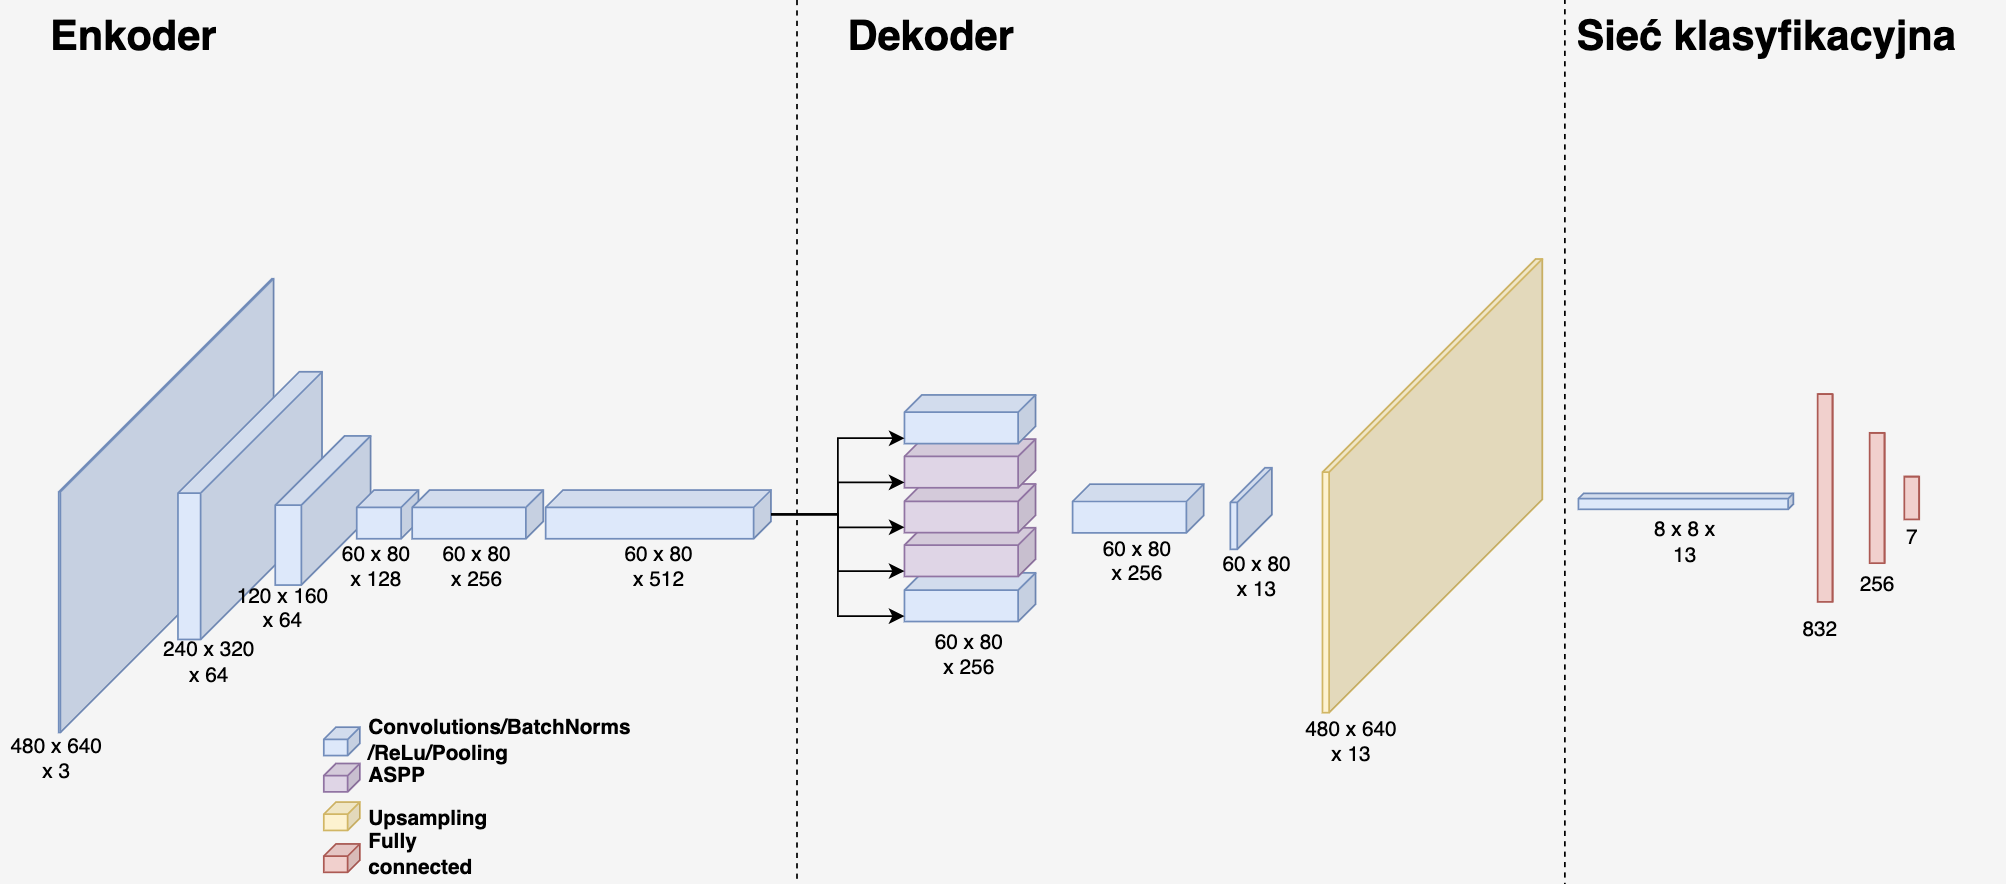
\includegraphics[width=\textwidth]{multitask-arch-seq-new.png}
    \caption{Architektura sieci szeregowej.}
    \label{fig:multitask-seq}
\end{figure}



\subsection{Zbiór  danych}
Dane są kluczową częścią głębokiego uczenia. Duży zbiór danych oznaczonych adnotacjami na poziomie pikseli jest potrzebny do wytrenowania wydajnego modelu segmentacji semantycznej. Typowe zestawy danych do segmentacji semantycznej to Cityscapes, PASCAL VOC i ADE20K. Podobnie w przypadku klasyfikacji sceny wymagany jest duży zbiór danych z odpowiednią informacją o etykiecie. Popularne zestawy danych do klasyfikacji scen obejmują NYUv2, SUN RGB-D, Matterport3D i ScanNet.
\subsubsection{Wybór zbioru danych}
Po prześledzeniu wielu zbiorów danych udało się sprostać wymaganiom pracy, uzyskując dwa podobne zbiory danych - \texttt{NYUv2} oraz \texttt{SUN RGBD}. Ostatecznie wybrano \texttt{NYUv2}. Trudno jednozczanie odpowiedzieć, który zbiór jest lepszy. Wykorzystano fakt cytowalności. Okazuje się, że \texttt{NYUv2} jest też chętniej cytowany niż \texttt{SUN RGBD} (rys. \ref{fig:sun-vs-nyu}), zatem to ten zbiór właśnie wybrano.

\begin{figure}[ht!]
    \centering
    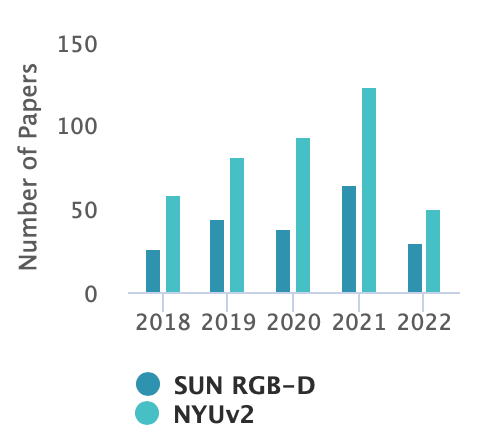
\includegraphics[width=0.5\textwidth]{img/stats-dataset.png}
    \caption[]{Szacowana liczba cytowań w latach 2018-2022 \href{https://paperswithcode.com/dataset/sun-rgb-d}{[paperswithcode.com]}}
    \label{fig:sun-vs-nyu}
\end{figure}
\subsection{Analiza zbioru danych}
Eksploracyjna analiza danych (ang. EDA) to proces eksploracji i zrozumienia cech zbioru danych przed zbudowaniem modelu. Jednym z głównych powodów, dla których proces ten jest ważny w wizji komputerowej to fakt, że może pomóc w identyfikacji problemów ze zbiorem danych, takich jak nieprawidłowe etykiety. Co więcej, może ono być również wykorzystane do identyfikacji skośnych rozkładów klas prowadzących do niesprawiedliwych prognoz. EDA może być również wykorzystana do określenia, które kroki przetwarzania wstępnego (ang. preprocessing), takie jak augmentacja, są niezbędne do poprawy wydajności modelu wizji komputerowej. Badając dane i rozumiejąc ich charakterystykę, możemy uzyskać głębsze ich zrozumienie i zidentyfikować wszelkie problemy, które należy rozwiązać przed zbudowaniem modelu.

EDA przeprowadzone na zbiorze NYUv2 dostarczyło wielu interesujących szczegółów. W zbiorze domyślnie znajduje się 795 przykładów trenujących oraz 654 przykładów testujących. Ze zbioru testowego wyodrębniono zbiór walidacyjny stanowiący 20\% zbioru testowego. Ponadto sprawdzono rozkład klas na przestrzeni całego zbioru danych.
W przypadku zadania segmentacji semantycznej do dyspozycji był wybór 894, 40 lub 13 klas przedmiotów. Im rozróżnialność była większa, tym większe okazywały się dysproporcje w rozkładzie. Histogramy dla 13 i 40 klas przedstawiono na rysunku \ref{fig:rozklad-segm}.
Podobna sytuacja miała miejsce dla zadania klasyfikacji z tą różnicą, iż scalania klas należało dokonać ręcznie. Taki krok był kluczowy, gdyż pierwotny rozkład był silnie zdominowany przez kilka klas.
Ostatecznie wybrano 13 klas dla klasyfikacji (rys. \ref{fig:7 klas dystrybucja}) oraz scalone 7 dla segmentacji (rys. \ref{fig:7 klas dystrybucja}).

\begin{figure}[ht!]
\centering
\begin{subfigure}[b]{0.49\textwidth}
\centering
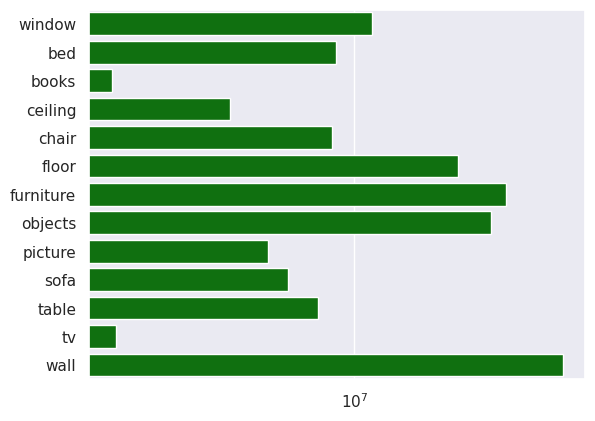
\includegraphics[width=\textwidth]{seg13.png}
\caption{Rozkład dla 13 klas.}
\label{fig:rozklad-13klas-seg}
\end{subfigure}
\hfill
\begin{subfigure}[b]{0.49\textwidth}
\centering
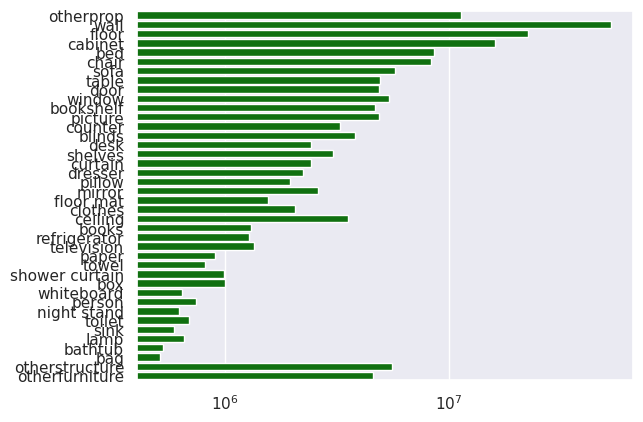
\includegraphics[width=\textwidth]{seg40.png}
\caption{Rozkład dla 40 klas.}
\label{fig:rozklad-40klas-seg}
\end{subfigure}
\caption[]{Porównanie rozkładu ilości pikseli dla zadania segmentacji semantycznej.}
\label{fig:rozklad-segm}
\end{figure}

\begin{figure}
\centering
\begin{subfigure}[b]{0.49\textwidth}
\centering
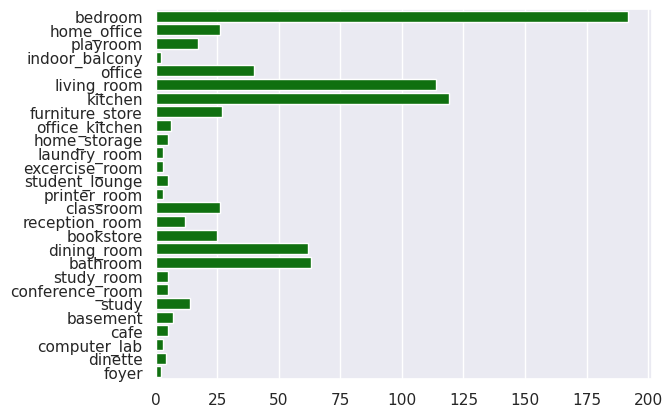
\includegraphics[width=\textwidth]{classification.png}
\caption{Oryginalny rozkład klas.}
\label{fig:27 klas dystrybucja}
\end{subfigure}
\hfill
\begin{subfigure}[b]{0.49\textwidth}
\centering
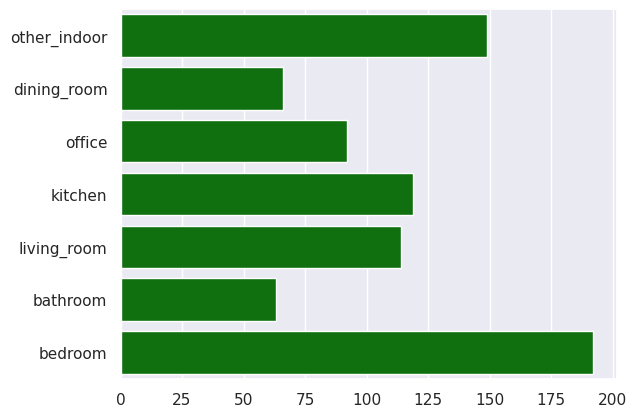
\includegraphics[width=\textwidth]{classification-merged.png}
\caption{Rozkład klas po scaleniu.}
\label{fig:7 klas dystrybucja}
\end{subfigure}
\caption[]{Porównanie rozkładu klas dla zadania klasyfikacji sceny.}
\end{figure}



% W celu łatwej oraz dokładniej ewaluaji 

% W celu lepsze ewaluacji uczenia wielozadaniowego zdecydowano uściślij wszystkie parametry sieci takie jak architekura jest ta sama zeby dało sie porownac nie

% nie ma sensu wszystkich scenariusz bo tak

% opisać że nie ma sensu porównywać 





























% Poza uczeniem łącznym zbadano też inne znane techniki uczenia jak finetuning.


% % * multitask Learning
% % * jednozadaniowe
% % * wielozadaniowe
% W celu realizacji zadania zdecydowano się na architekturę (najbliższą Y-Netu) o wspólnym enkoderze i o osobnych głowach, służących do egzekwowania konkretnych zadań (rys. \ref{fig:cep_arch}). Decyzja podyktowana była względnie prostą implementacją rozszerzenia wielu modeli segmentacji semantycznej o dodatkową głowę klasyfikacyjną. Co więcej stwierdzono, że ograniczenie się tylko do jednego backbone'u jest niesłychanie korzystne, gdyż znacząco ogranicza ilość parametrów sieci, co bezpośrednio przekłada się m.in. na czas inferencji. Należy zwrócić uwagę na fakt, iż właściwie zdecydowana większość parametrów znajduje się własnie w enkoderze.

% Mając na uwadze, że symultaniczne uczenie może negatywnie wpływać na jakość uczenia obu zadań, eksperymenty przeprowadzono etapowo. Pierwszym etapem było uczenie jednozadaniowe. Eksperymenty polegały na sprawdzeniu jakości segmentacji oraz klasyfikacji osobno. Wykorzystano do tego tę samą archtekturę, która używana była poźniej w drugim etapie. Mianowicie, mając dwie głowy każdorazowo zamrażano głowę nie biorącą udziału w uczeniu (rys. \ref{fig:arch-scene-seg}). Zapewnia to pewność posiadania tej samej architektury, a w szczególności rzetelne porównanie z etapem uczenia wielozadaniowego.

% Drugim etapem było przeprowadzenie eksperymentów w uczeniu wielozadaniowym (rys. \ref{fig:arch-full}). Funkcja celu zdefiniowana była jako suma wartości funkcji celów dla obu zadań. W wyniku progpagacji wstecznej wagi aktualizowane były zgodnie z zagregowaną stratą.

% Ostatecznie porównano jakość na przesztreni obu etapów.

% \begin{figure}[ht!]
%     \centering
%     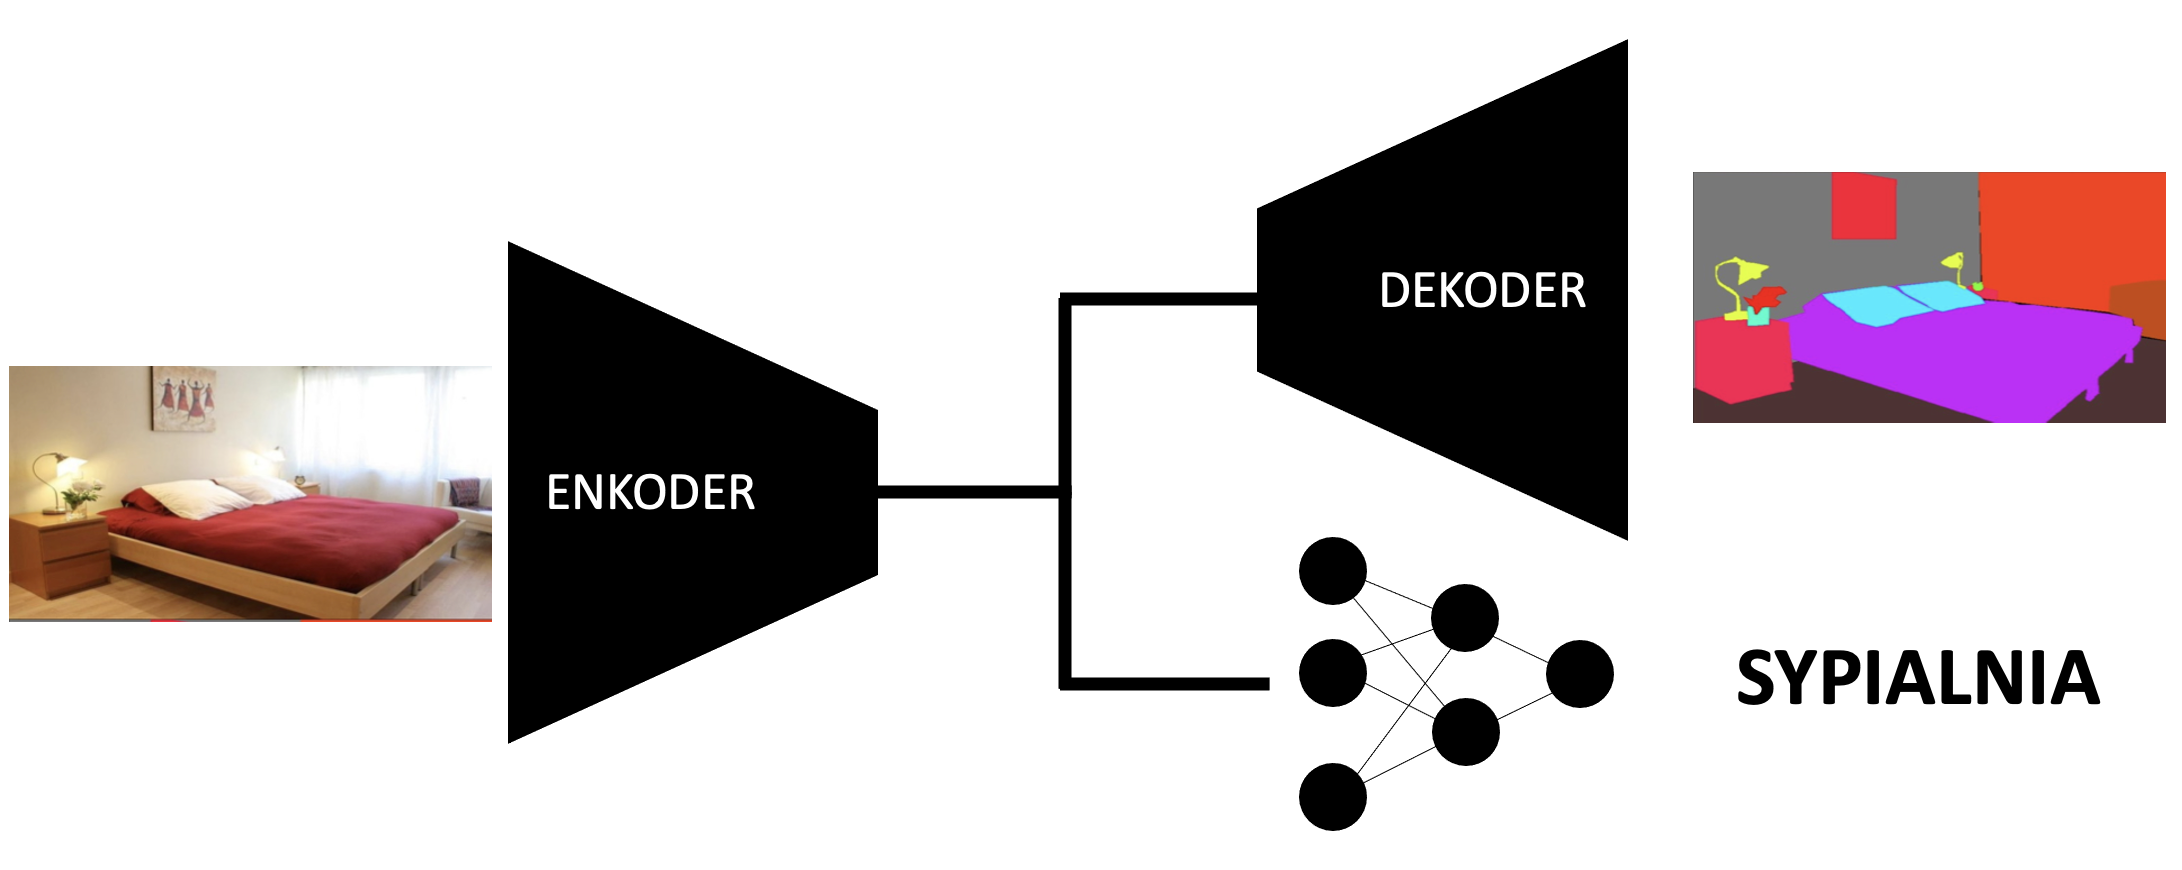
\includegraphics[width=0.75\textwidth]{cep_arch.png}
%     \caption{Architektura sieci zastosowana w pracy inżynierskiej.}
%     \label{fig:cep_arch}
% \end{figure}

% \begin{figure}[ht!]
%     \centering
%     \begin{subfigure}[b]{0.49\textwidth}
%         \centering
%         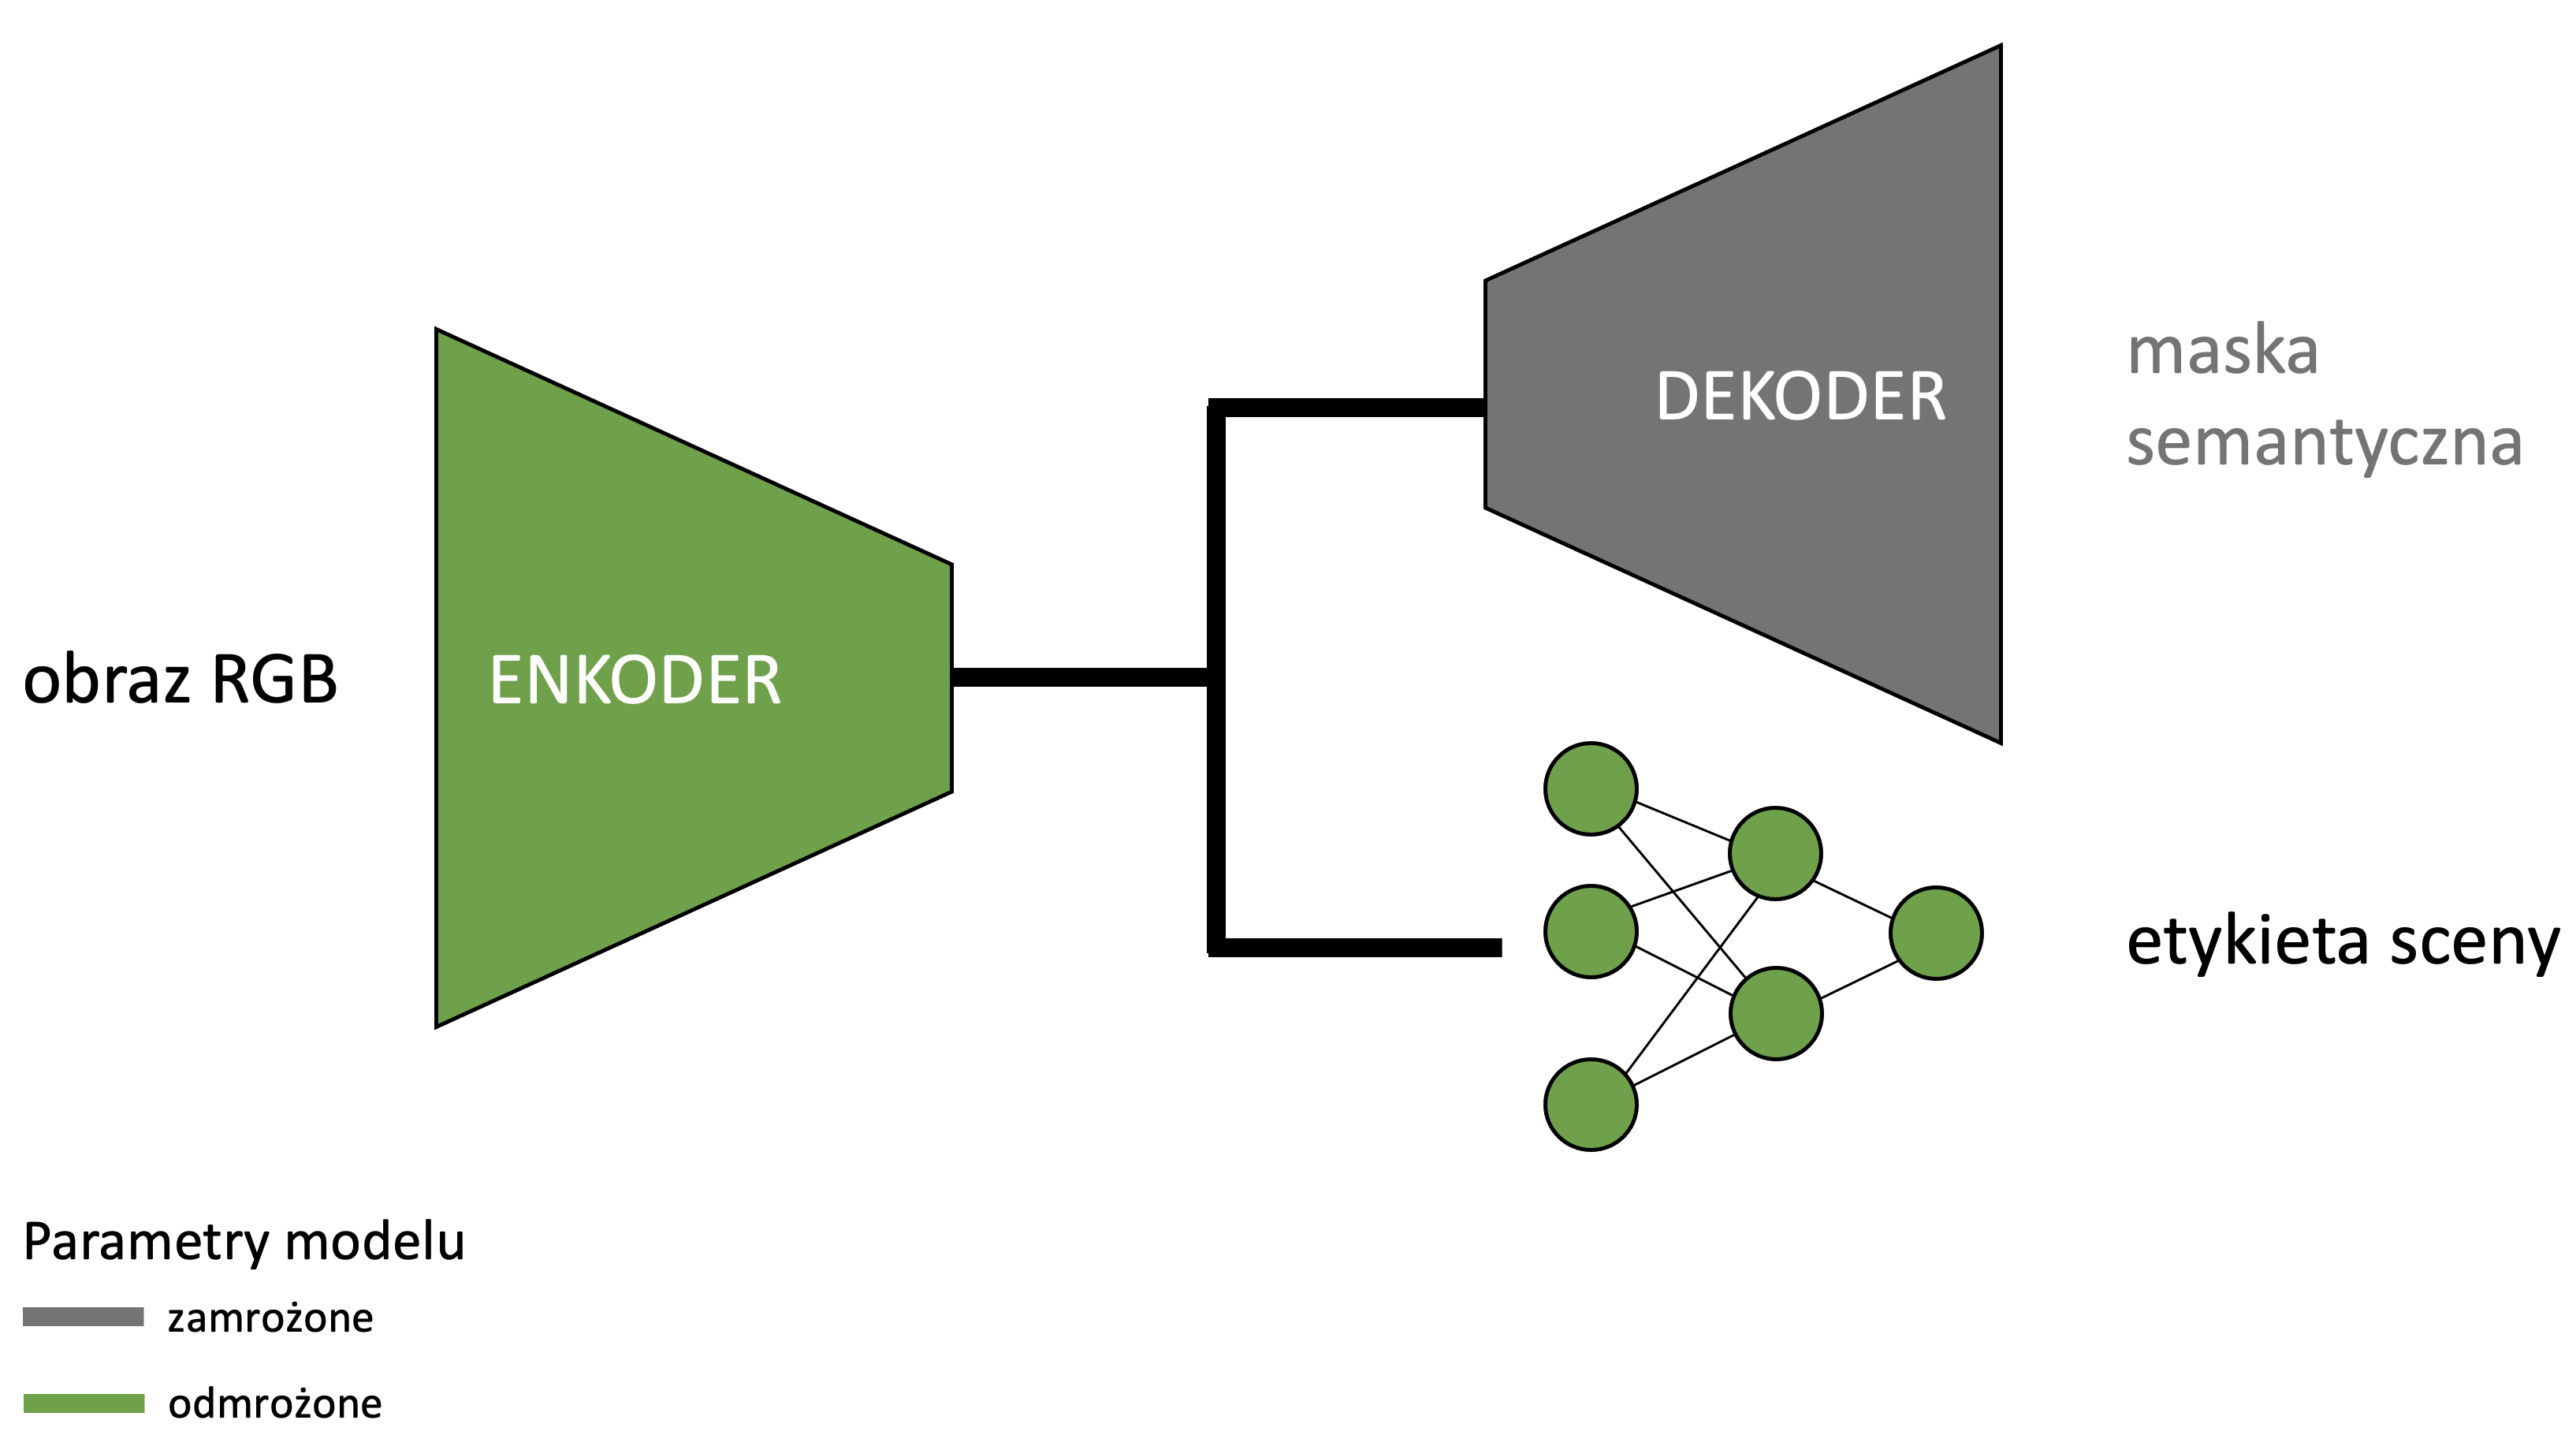
\includegraphics[width=\textwidth]{arch:scene.png}
%         \caption{Architektura sieci wyłącznie w zadaniu klasyfikacji.}
%     \end{subfigure}
%     \hfill
%     \begin{subfigure}[b]{0.49\textwidth}
%         \centering
%         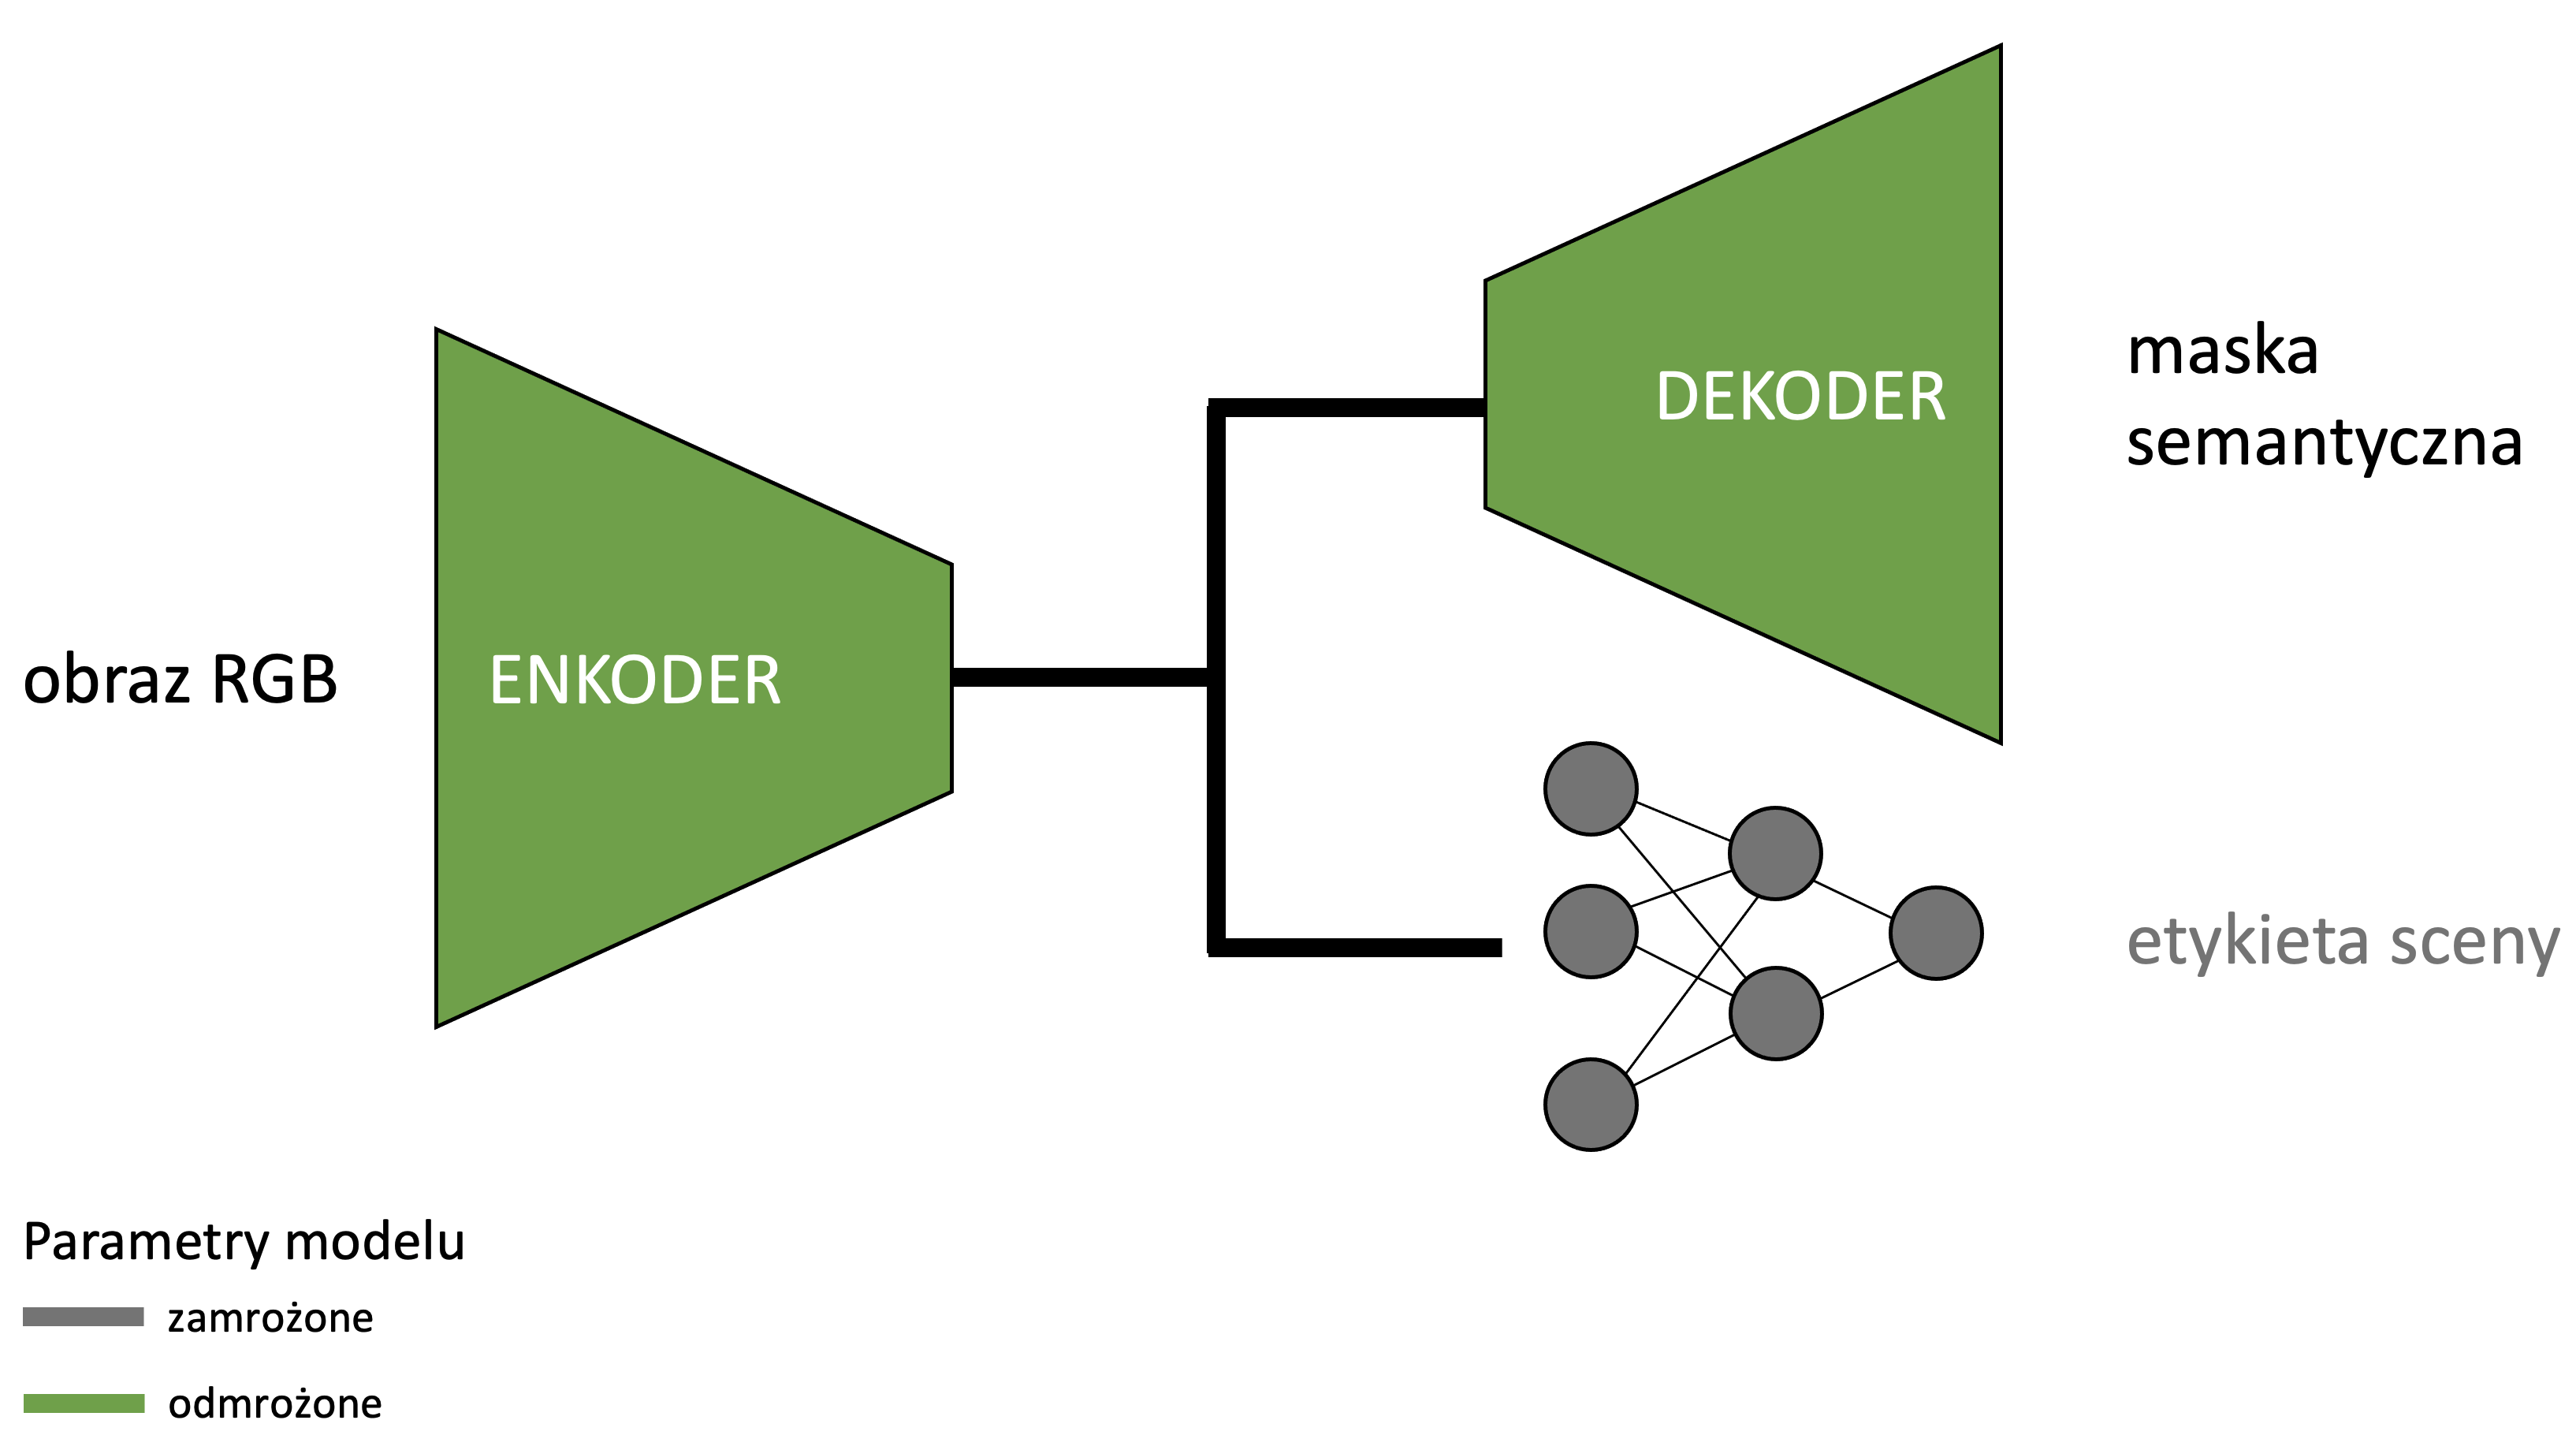
\includegraphics[width=\textwidth]{arch:seg.png}
%         \caption{Architektura sieci wyłącznie w zadaniu segmentacji semantycznej.}
%     \end{subfigure}
%     \caption[]{Podejście jednozadaniowe.}
%     \label{fig:arch-scene-seg}
% \end{figure}

% \begin{figure}[ht!]
%     \centering
%     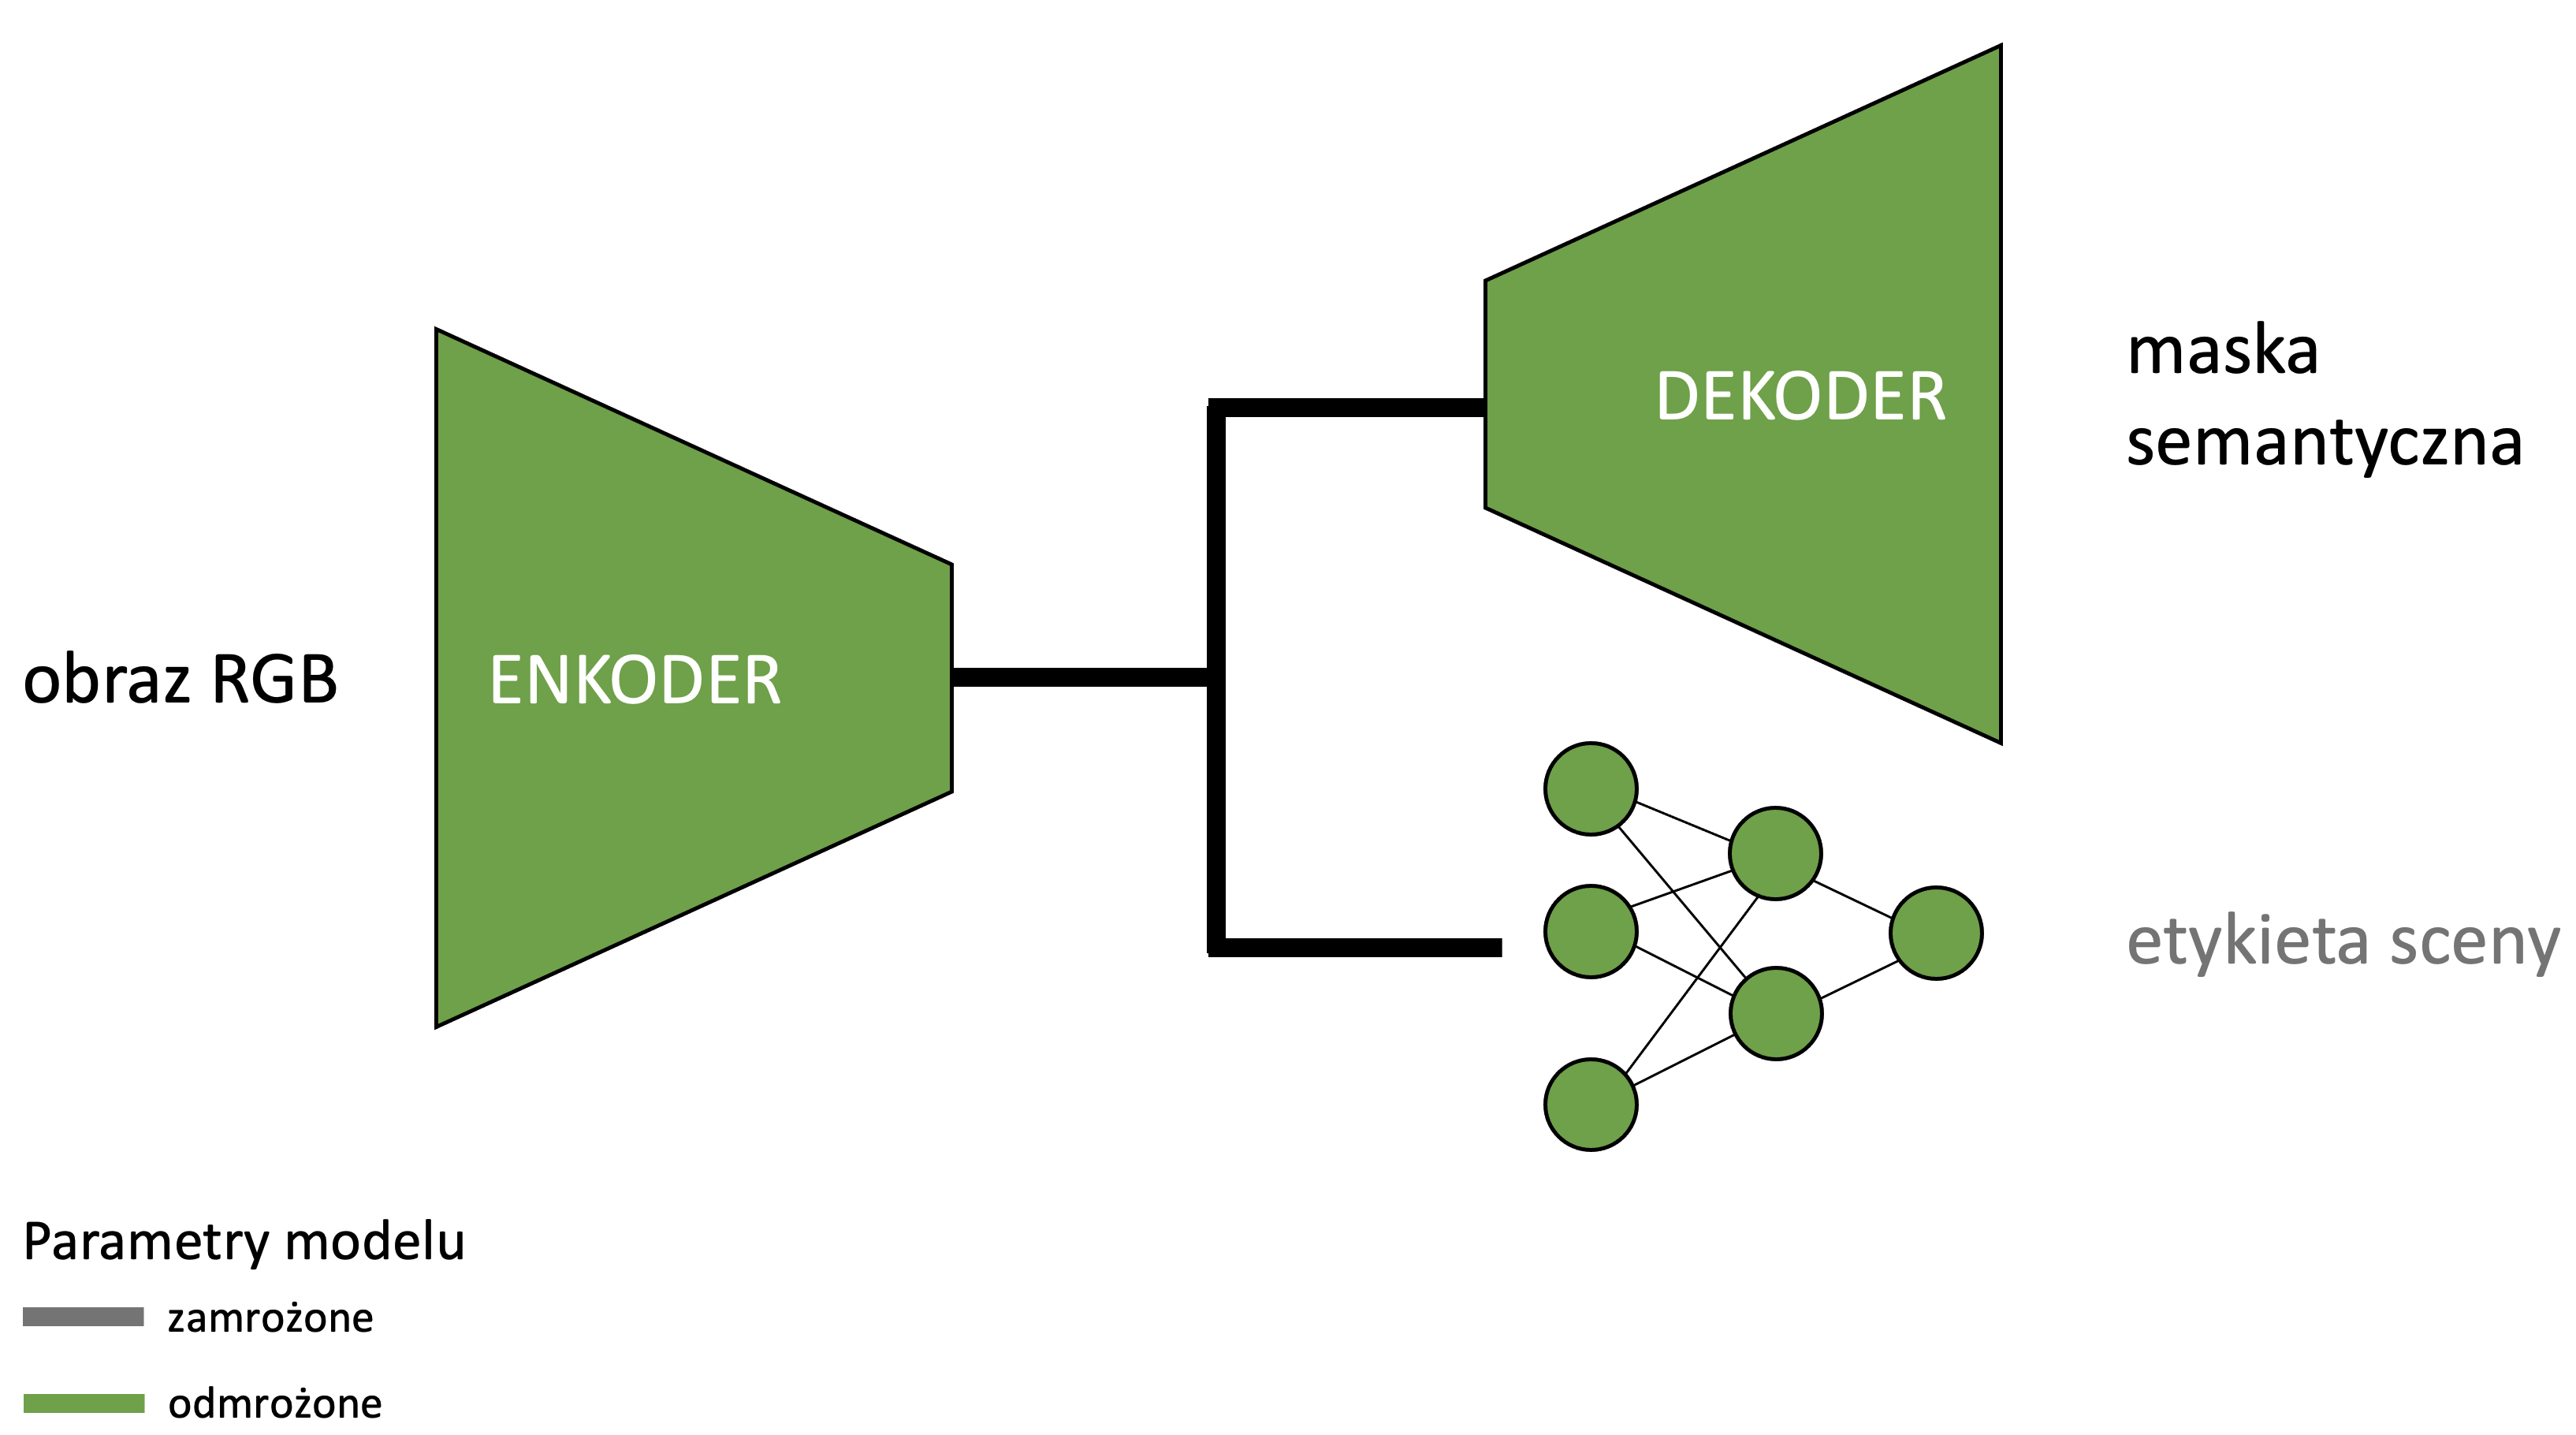
\includegraphics[width=0.75\textwidth]{arch:full.png}
%     \caption{Architektura sieci jako uczenie wielozadaniowego.}
%     \label{fig:arch-full}
% \end{figure}